% Where Is the Mug? -- object poses from the depth cameras (pose-estimation steps 1-9)
% Build: tectonic -X compile pose_estimation_guide.tex   (figures/ is written by make_figures.py)
\documentclass[11pt,a4paper]{article}

\usepackage[margin=2.1cm,headheight=14pt]{geometry}
\usepackage{lmodern}
\usepackage[T1]{fontenc}
\usepackage{microtype}
\usepackage{xcolor}
\usepackage{graphicx}
\usepackage{amsmath}
\usepackage{tikz}
\usetikzlibrary{arrows.meta,positioning,shapes.geometric,shapes.misc,fit,backgrounds,calc,decorations.pathreplacing}
\usepackage[most]{tcolorbox}
\usepackage{booktabs}
\usepackage{tabularx}
\usepackage{enumitem}
\usepackage{fontawesome5}
\usepackage{fancyhdr}
\usepackage{titlesec}
\usepackage{float}
\usepackage{needspace}
\usepackage[hidelinks]{hyperref}

% ---------------------------------------------------------------- colours (as the perception guide)
\definecolor{ink}{HTML}{1F2933}
\definecolor{sky}{HTML}{2B6CB0}
\definecolor{skylight}{HTML}{EBF4FF}
\definecolor{leaf}{HTML}{2F855A}
\definecolor{leaflight}{HTML}{E6FFFA}
\definecolor{sun}{HTML}{B7791F}
\definecolor{sunlight}{HTML}{FFFAEB}
\definecolor{rose}{HTML}{C53030}
\definecolor{roselight}{HTML}{FFF5F5}
\definecolor{grape}{HTML}{6B46C1}
\definecolor{stone}{HTML}{718096}

\color{ink}
\hypersetup{colorlinks=true,linkcolor=sky,urlcolor=sky}
\titleformat{\section}{\Large\bfseries\color{sky}}{\thesection}{0.8em}{}[{\color{sky!40}\titlerule[1pt]}]
\titleformat{\subsection}{\large\bfseries\color{ink}}{\thesubsection}{0.7em}{}
\pagestyle{fancy}
\fancyhf{}
\fancyhead[L]{\small\color{stone}\faCube\ \ Where Is the Mug?}
\fancyhead[R]{\small\color{stone}perception/pose-estimation}
\fancyfoot[C]{\small\color{stone}\thepage}
\renewcommand{\headrulewidth}{0.4pt}
\setlist{itemsep=2pt,topsep=4pt}
\newcommand{\sectionbreak}{\needspace{22\baselineskip}}
\newcommand{\subsectionbreak}{\needspace{16\baselineskip}}

\newtcolorbox{eli5}{enhanced,colback=sunlight,colframe=sun,boxrule=0.8pt,arc=3mm,
  title={\faChild\ \ In plain words},fonttitle=\bfseries,coltitle=white}
\newtcolorbox{changeit}{enhanced,before upper={\raggedright},colback=leaflight,colframe=leaf,boxrule=0.8pt,arc=3mm,
  title={\faWrench\ \ Where it lives in the code},fonttitle=\bfseries}
\newtcolorbox{careful}{enhanced,before upper={\raggedright},colback=roselight,colframe=rose,boxrule=0.8pt,arc=3mm,
  title={\faExclamationTriangle\ \ Careful},fonttitle=\bfseries}
\newtcolorbox{keyidea}{enhanced,before upper={\raggedright},colback=skylight,colframe=sky,boxrule=0.8pt,arc=3mm,
  title={\faLightbulb\ \ Key idea},fonttitle=\bfseries}
\newtcolorbox{cmd}[1][]{enhanced,breakable,colback=ink!92,colframe=ink,coltext=white,boxrule=0pt,
  arc=2mm,left=6pt,right=6pt,top=4pt,bottom=4pt,fontupper=\ttfamily\small,#1}
\newcommand{\code}[1]{\texttt{\detokenize{#1}}}

\tikzset{
  >={Stealth[length=2.6mm]},
  box/.style={draw=#1,fill=#1!8,rounded corners=3pt,thick,align=center,inner sep=6pt,font=\small},
  box/.default=sky,
  flow/.style={->,thick,draw=ink!70},
  lbl/.style={font=\scriptsize,text=ink!80,align=center},
}

\begin{document}

% ================================================================ TITLE
\begin{titlepage}
\centering
\vspace*{1.2cm}
{\color{sky}\fontsize{30}{36}\selectfont\bfseries Where Is the Mug?\par}
\vspace{0.4cm}
{\Large\color{stone} Object poses from the depth cameras:\\[2pt]
what we built in steps 1--9, why, and what it means for the supervisor\par}
\vspace{1.3cm}
\begin{tikzpicture}[scale=0.95]
  \node[box=grape,minimum width=2.4cm,minimum height=1.4cm] (mask) at (0,0) {\faImage\\[2pt]\textbf{Mask}\\\scriptsize SAM 3};
  \node[box=sky,minimum width=2.4cm,minimum height=1.4cm] (pts) at (3.3,0) {\faBraille\\[2pt]\textbf{3D points}\\\scriptsize depth + calibration};
  \node[box=sun,minimum width=2.4cm,minimum height=1.4cm] (fit) at (6.6,0) {\faDatabase\\[2pt]\textbf{Cylinder}\\\scriptsize fitted per camera};
  \node[box=leaf,minimum width=2.4cm,minimum height=1.4cm] (pose) at (9.9,0) {\faCrosshairs\\[2pt]\textbf{Pose}\\\scriptsize base, axis, trust};
  \draw[flow] (mask) -- (pts);
  \draw[flow] (pts) -- (fit);
  \draw[flow] (fit) -- (pose);
\end{tikzpicture}
\vspace{1.2cm}

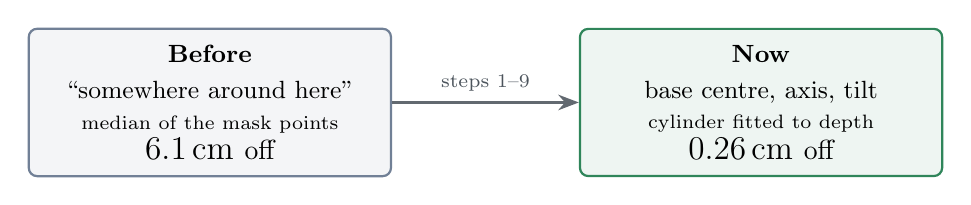
\begin{tikzpicture}
  \node[box=stone,minimum width=4.6cm] (before) at (0,0) {\textbf{Before}\\[2pt]``somewhere around here''\\\scriptsize median of the mask points\\\large 6.1\,cm\ \normalsize off};
  \node[box=leaf,minimum width=4.6cm] (after) at (7,0) {\textbf{Now}\\[2pt]base centre, axis, tilt\\\scriptsize cylinder fitted to depth\\\large 0.26\,cm\ \normalsize off};
  \draw[flow,line width=1.4pt] (before) -- node[lbl,above]{steps 1--9} (after);
\end{tikzpicture}
\vfill
\begin{keyidea}
The robot can now say \emph{where the bottom of the mug is} to within a few millimetres,
\emph{which way it points} to about a degree, \emph{where its handle is}, and \emph{where on the
rack's peg a hung mug must end up}, using only its cameras and its own joint sensors. It
already stops the gripper opening on a mug that lies on its side. Behind a setting, it can
also aim the arm at the mug and the rack.
\end{keyidea}
\vspace{0.4cm}
{\color{stone}Olusola --- perception and object grounding \quad$\cdot$\quad 2026-11-05\par}
\end{titlepage}

\tableofcontents
\newpage

% ================================================================ 1
\section{Why the robot needs a pose}

Until now, ``where is the mug'' was answered with one number per axis: the \textbf{median}
of the 3D points inside the mug's mask. That is a fine ``roughly here'', but it has two problems
that matter for the supervisor.

\begin{center}
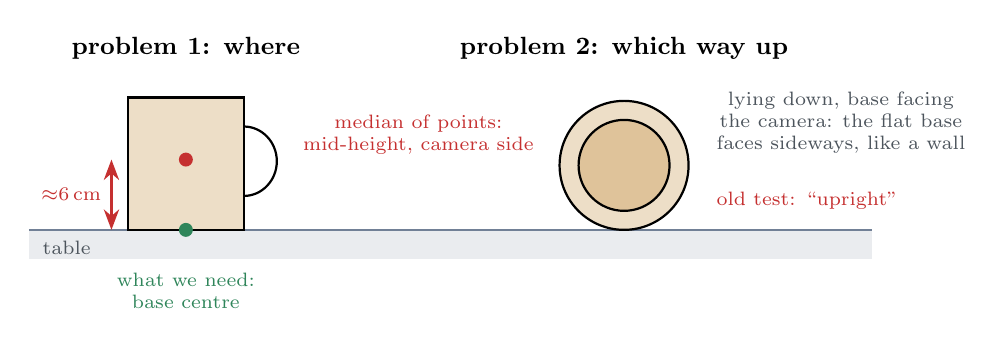
\begin{tikzpicture}[scale=1.05]
  % table
  \fill[stone!15] (-0.6,0) rectangle (9.6,-0.35);
  \draw[stone,thick] (-0.6,0) -- (9.6,0);
  \node[lbl,anchor=north west] at (-0.55,-0.02) {table};
  % mug A upright
  \draw[thick,fill=sun!25] (0.6,0) rectangle (2.0,1.6);
  \draw[thick] (2.0,1.25) arc (90:-90:0.4 and 0.42);
  \fill[rose] (1.3,0.85) circle (2.4pt);
  \node[lbl,text=rose,anchor=west] at (2.6,1.15) {median of points:\\mid-height, camera side};
  \fill[leaf] (1.3,0) circle (2.4pt);
  \node[lbl,text=leaf,anchor=north] at (1.3,-0.4) {what we need:\\base centre};
  \draw[<->,rose,thick] (0.4,0) -- node[lbl,left,text=rose]{$\approx$6\,cm} (0.4,0.85);
  % mug B end-on toppled
  \begin{scope}[shift={(6.6,0)}]
    \draw[thick,fill=sun!25] (0,0.78) ellipse (0.78 and 0.78);
    \draw[thick,fill=sun!45] (0,0.78) ellipse (0.55 and 0.55);
    \node[lbl,anchor=west] at (1.0,1.3) {lying down, base facing\\the camera: the flat base\\faces sideways, like a wall};
    \node[lbl,text=rose,anchor=west] at (1.0,0.35) {old test: ``upright''};
  \end{scope}
  \node[font=\bfseries\small] at (1.3,2.2) {problem 1: where};
  \node[font=\bfseries\small] at (6.6,2.2) {problem 2: which way up};
\end{tikzpicture}
\end{center}

\begin{enumerate}
  \item \textbf{Position.} The median lands about half a mug height above the base and is pulled
        towards the camera. On seeds 0--4 it was \textbf{6.1\,cm} from the true base centre for
        mugs on the table. A grasp or a placement aimed there is aimed at air.
  \item \textbf{Orientation.} ``Safe to open the gripper'' (\code{release_ready}) checked that the
        mug's visible surface faces sideways, as an upright mug's wall does. A mug lying with its
        base towards the camera fools it, because a flat base also faces sideways. On held-out
        seed 6 this produced \textbf{25 wrong ``safe to release''} answers.
\end{enumerate}

\begin{eli5}
Knowing \emph{where a cup is} is not enough to pick it up or put it down. You need to know
where its bottom is and whether it is standing or lying. A pose is those two things together.
\end{eli5}

\subsection{The rules we kept}
\begin{center}
\begin{tikzpicture}
  \node[box=leaf,text width=4.3cm,minimum height=2.3cm,align=left] (ok) at (0,0) {\textbf{\faCheck\ Allowed at runtime}\\[3pt]
    \small RGB-D images and their calibration\\ SAM 3 masks\\ the robot's own measured joints,\\hand poses and grippers};
  \node[box=rose,text width=4.3cm,minimum height=2.3cm,align=left] (no) at (5.2,0) {\textbf{\faTimes\ Offline only}\\[3pt]
    \small simulator object poses (labels)\\ the mug meshes\\ which mug model was loaded};
  \node[box=sky,text width=4.3cm,minimum height=2.3cm,align=left] (rule) at (10.4,0) {\textbf{\faBalanceScale\ How we decide}\\[3pt]
    \small \emph{unknown} beats a guess\\ precision before recall\\ tune on seeds 0--4, check on others};
\end{tikzpicture}
\end{center}

% ================================================================ 2
\section{The whole pipeline on one page}

\begin{center}
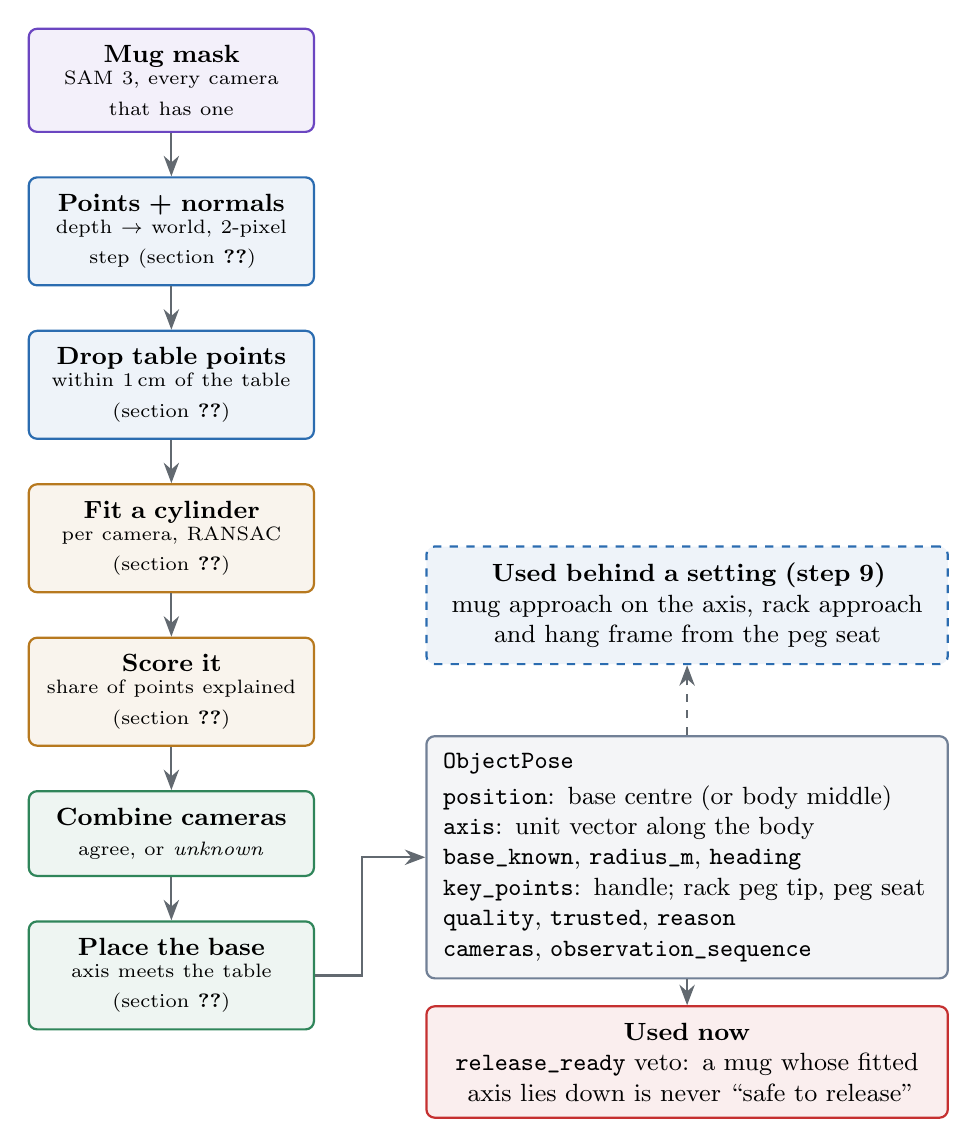
\begin{tikzpicture}[node distance=0.55cm]
  \node[box=grape,text width=3.2cm] (m) {\textbf{Mug mask}\\\scriptsize SAM 3, every camera\\that has one};
  \node[box=sky,text width=3.2cm,below=of m] (p) {\textbf{Points + normals}\\\scriptsize depth $\to$ world, 2-pixel\\step (section~\ref{sec:points})};
  \node[box=sky,text width=3.2cm,below=of p] (t) {\textbf{Drop table points}\\\scriptsize within 1\,cm of the table\\(section~\ref{sec:shadow})};
  \node[box=sun,text width=3.2cm,below=of t] (f) {\textbf{Fit a cylinder}\\\scriptsize per camera, RANSAC\\(section~\ref{sec:fit})};
  \node[box=sun,text width=3.2cm,below=of f] (q) {\textbf{Score it}\\\scriptsize share of points explained\\(section~\ref{sec:trust})};
  \node[box=leaf,text width=3.2cm,below=of q] (c) {\textbf{Combine cameras}\\\scriptsize agree, or \emph{unknown}};
  \node[box=leaf,text width=3.2cm,below=of c] (b) {\textbf{Place the base}\\\scriptsize axis meets the table\\(section~\ref{sec:base})};
  \foreach \a/\b in {m/p,p/t,t/f,f/q,q/c,c/b} \draw[flow] (\a) -- (\b);

  \node[box=stone,text width=6.2cm,anchor=west,align=left] (o) at ($(b.east)+(1.4,1.5)$) {\textbf{\code{ObjectPose}}\\[2pt]\raggedright\small
    \code{position}: base centre (or body middle)\\
    \code{axis}: unit vector along the body\\
    \code{base_known}, \code{radius_m}, \code{heading}\\
    \code{key_points}: handle; rack peg tip, peg seat\\
    \code{quality}, \code{trusted}, \code{reason}\\
    \code{cameras}, \code{observation_sequence}};
  \draw[flow] (b.east) -- ++(0.6,0) |- (o.west);

  \node[box=rose,text width=6.2cm,anchor=west] (r) at ($(o.west)+(0,-2.6)$) {\textbf{Used now}\\\small \code{release_ready} veto: a mug whose fitted\\axis lies down is never ``safe to release''};
  \node[box=sky,text width=6.2cm,anchor=west,dashed] (n) at ($(o.west)+(0,3.2)$) {\textbf{Used behind a setting (step 9)}\\\small mug approach on the axis, rack approach\\and hang frame from the peg seat};
  \draw[flow] (o) -- (r);
  \draw[flow,dashed] (o) -- (n);
\end{tikzpicture}
\end{center}

\begin{changeit}
\begin{itemize}[leftmargin=*]
  \item \code{harness/perception/object_pose.py}: everything in the left column, plus \code{ObjectSpec} and \code{ObjectPose}.
  \item \code{harness/perception/rgbd.py}: \code{RGBDCamera.surface_points_and_normals}.
  \item \code{harness/perception/grounding.py}: \code{RGBDPerceptionProvider._mug_pose} runs it once per observation; the result is \code{GroundingResult.mug_pose}.
  \item \code{development/replays/perception_evaluation.py}: pose metrics against the labels.
\end{itemize}
\end{changeit}

\subsection{Category, not model}
The fitter knows a mug only as an \code{ObjectSpec}: ``a cylinder with radius 3--7\,cm and height
6--14\,cm that stands on the table''. It never looks up which of RoboTwin's ten mug meshes was
loaded. A different mug, or a bottle, needs a new spec line, not new code. This was one of the
decisions in the plan: no mesh files at runtime.

% ================================================================ 3
\section{Step 1: measuring before improving}

Every change here was judged by numbers from the existing evaluator, which replays saved frames
through the real runtime code and compares with the simulator's labels. We added pose metrics:
axis error, base position error, upright/toppled mistakes, coverage, and \textbf{confident wrong
poses} (trusted, but off by more than 20\textdegree{} or 3\,cm). That last one is the pose
version of a false ``true''.

\subsection{The answer key was wrong by two centimetres}
The first run gave a stubborn 1.9\,cm horizontal error on \emph{every} mug on the table, with
almost no spread. A constant error is usually a definition problem, not a perception one.

\begin{center}
\begin{minipage}{0.47\textwidth}
\centering
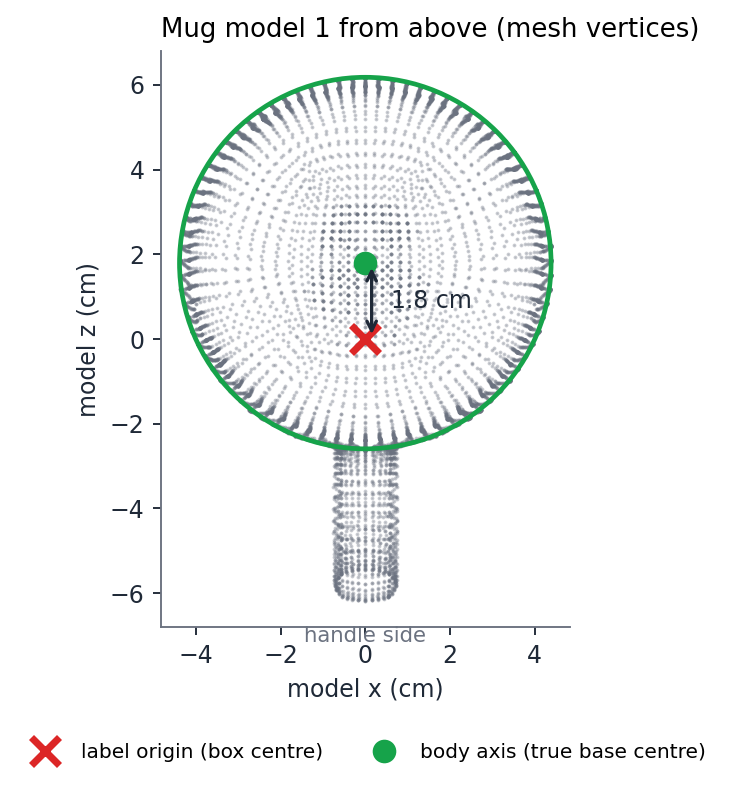
\includegraphics[width=\textwidth]{figures/mesh_offset.png}
\end{minipage}\hfill
\begin{minipage}{0.48\textwidth}
\begin{careful}
The label's \code{mug.pose} origin is the centre of a box that \emph{includes the handle}. The
mug's body axis sits \textbf{1.6--2.6\,cm} away from it, on the side away from the handle,
depending on the model.
\end{careful}
\small
What we did (offline only):
\begin{itemize}[leftmargin=*]
  \item measured each model's offset from its mesh (\code{MUG_MODELS});
  \item recognised the episode's model from its handle point, which is different for every model;
  \item moved the truth onto the body axis (\code{true_mug_base});
  \item made new captures record \code{mug.model_id} directly.
\end{itemize}
Error after the fix: \textbf{0.26\,cm}.
\end{minipage}
\end{center}

\subsection{Which way is ``up'' for a mug model}
The meshes stand along their \textbf{+y} axis. The task spawns them turned 90\textdegree{} about
x, so +y points up in the world. The truth axis is therefore $R\,[0,1,0]^\top$, not the
quaternion's z axis as the first draft of the plan said.

\begin{center}
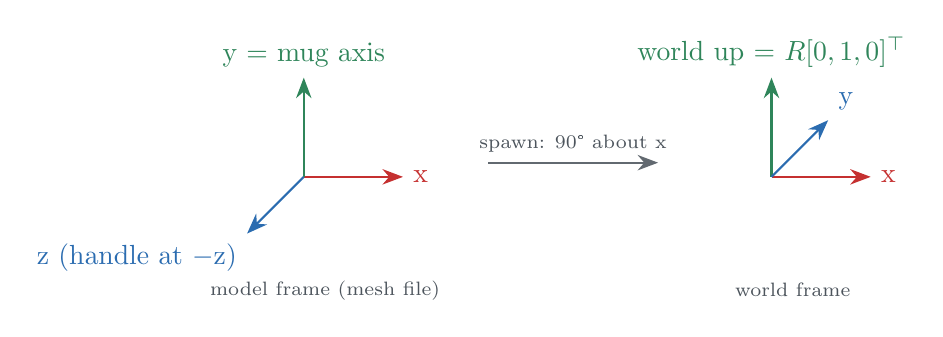
\begin{tikzpicture}[scale=0.9]
  \begin{scope}
    \draw[->,thick,rose] (0,0) -- (1.4,0) node[right]{x};
    \draw[->,thick,leaf] (0,0) -- (0,1.4) node[above]{y = mug axis};
    \draw[->,thick,sky] (0,0) -- (-0.8,-0.8) node[below left]{z (handle at $-$z)};
    \node[lbl] at (0.3,-1.6) {model frame (mesh file)};
  \end{scope}
  \draw[flow] (2.6,0.2) -- node[lbl,above]{spawn: 90\textdegree{} about x} (5.0,0.2);
  \begin{scope}[shift={(6.6,0)}]
    \draw[->,thick,rose] (0,0) -- (1.4,0) node[right]{x};
    \draw[->,thick,leaf] (0,0) -- (0,1.4) node[above]{world up = $R[0,1,0]^\top$};
    \draw[->,thick,sky] (0,0) -- (0.8,0.8) node[above right]{y};
    \node[lbl] at (0.3,-1.6) {world frame};
  \end{scope}
\end{tikzpicture}
\end{center}

% ================================================================ 4
\section{Step 2: from depth to points and normals}\label{sec:points}

Each mask pixel with a depth becomes a world point (as before). We also need its
\textbf{surface normal}: which way the surface faces. The normal at a pixel comes from the
depth of its neighbours left/right and up/down.

\begin{center}
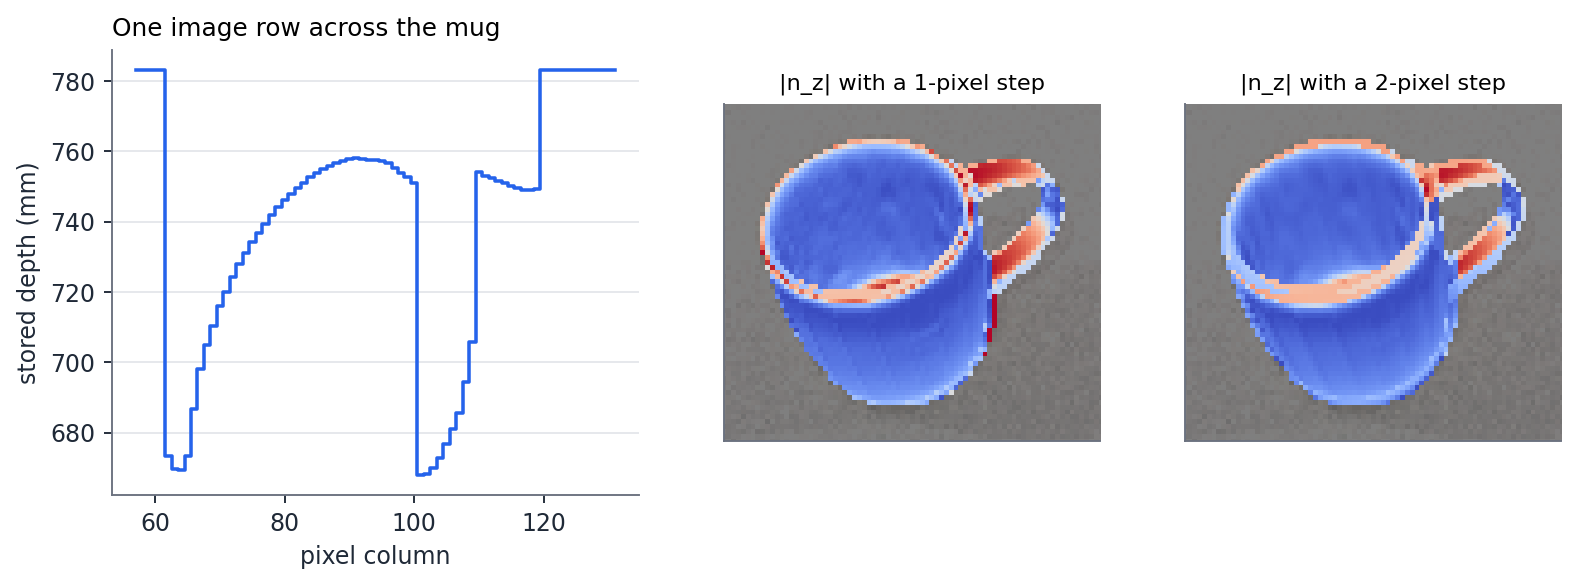
\includegraphics[width=\textwidth]{figures/depth_steps.png}
\end{center}

\begin{itemize}
  \item \textbf{Depth is stored in whole millimetres} (left: the staircase). Neighbours one pixel
        apart often differ by exactly 0 or 1\,mm, which makes normals jumpy. Measuring across
        \textbf{two pixels} on each side averages that rounding out; the wall colour is a little
        more even on the right. We did not run a separate test of one step against the other.
  \item \textbf{A bug we hit:} pixels next to an edge are skipped when neighbouring depths jump
        by more than 1\,cm. With the wider step, the two neighbours are 4 pixels apart, so a
        steep but smooth surface also ``jumps''. A toppled mug kept only \textbf{109 of its 1618
        mask pixels}. The limit now grows with the step.
\end{itemize}

\begin{changeit}
\code{RGBDCamera.surface_points_and_normals(mask, step_px=...)} returns world points and unit
normals (turned to face the camera). The old \code{vertical_normal_components} now calls it, so
the existing surface test is unchanged.
\end{changeit}

% ================================================================ 5
\section{Step 3: fitting a cylinder}\label{sec:fit}

A mug's body is close to a cylinder. A cylinder has a simple property we can test point by point:

\begin{keyidea}
On the curved wall, every surface normal is \textbf{perpendicular to the axis} and \textbf{points
at the axis}. Two wall normals are enough to guess the axis (their cross product), and their
lines meet at the centre.
\end{keyidea}

\begin{center}
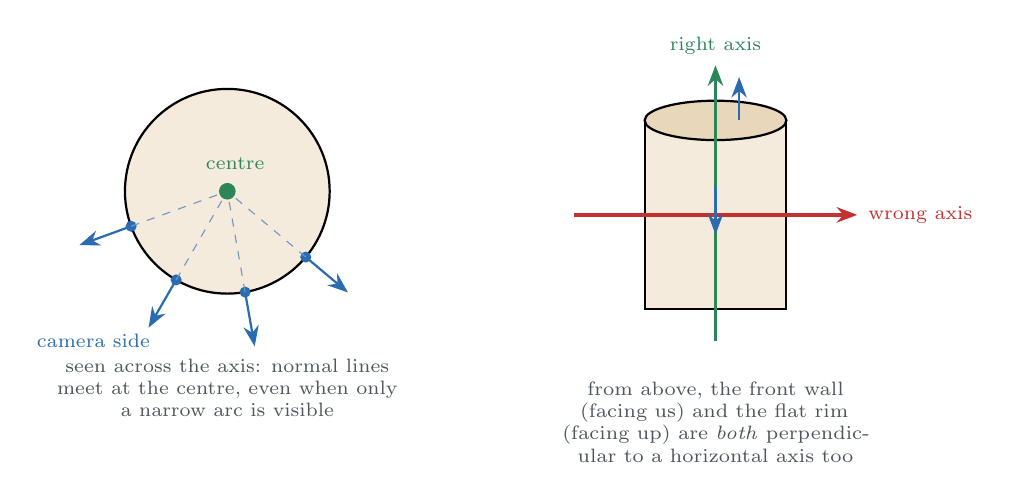
\begin{tikzpicture}[scale=1.0]
  % cross-section
  \begin{scope}
    \draw[thick,fill=sun!15] (0,0) circle (1.3);
    \foreach \ang in {200,240,280,320} {
      \fill[sky] (\ang:1.3) circle (2pt);
      \draw[->,thick,sky] (\ang:1.3) -- (\ang:2.0);
      \draw[dashed,sky!70] (\ang:1.3) -- (0,0);
    }
    \fill[leaf] (0,0) circle (3pt);
    \node[lbl,text=leaf] at (0.1,0.35) {centre};
    \node[lbl] at (0,-2.5) {seen across the axis: normal lines\\meet at the centre, even when only\\a narrow arc is visible};
    \node[lbl,text=sky] at (-1.7,-1.9) {camera side};
  \end{scope}
  % hypothesis test
  \begin{scope}[shift={(6.2,-0.3)}]
    \draw[thick,fill=sun!15] (-0.9,-1.2) rectangle (0.9,1.2);
    \draw[thick,fill=sun!30] (0,1.2) ellipse (0.9 and 0.25);
    \draw[->,leaf,line width=1.4pt] (0,-1.6) -- (0,1.9) node[above,lbl,text=leaf]{right axis};
    \draw[->,rose,line width=1.4pt] (-1.8,0.0) -- (1.8,0.0) node[right,lbl,text=rose]{wrong axis};
    \draw[->,thick,sky] (0,0.35) -- (0,-0.25);
    \draw[->,thick,sky] (0.3,1.2) -- (0.3,1.75);
    \node[lbl,text width=4.2cm,anchor=north] at (0,-2.0) {from above, the front wall (facing us)
      and the flat rim (facing up) are \emph{both} perpendicular to a horizontal axis too};
  \end{scope}
\end{tikzpicture}
\end{center}

\subsection{The trap, and how we avoided it}
Our first version scored an axis guess only by ``how many normals are perpendicular to it''. From
an elevated camera that let a \textbf{horizontal} axis explain an upright mug's front wall and
rim (right drawing). In the first test on seeds 0--4, more than a dozen per-camera fits of
upright mugs came out about 90\textdegree{} wrong.

The fix is to test a \emph{whole cylinder}, not just a direction. Each random pair of points
fixes the axis, the centre (where their normal lines meet) and the radius; a point only counts
if its normal fits \emph{and} it lies on that cylinder's surface (within 4\,mm). Wrong axes stop
adding up.

\begin{center}
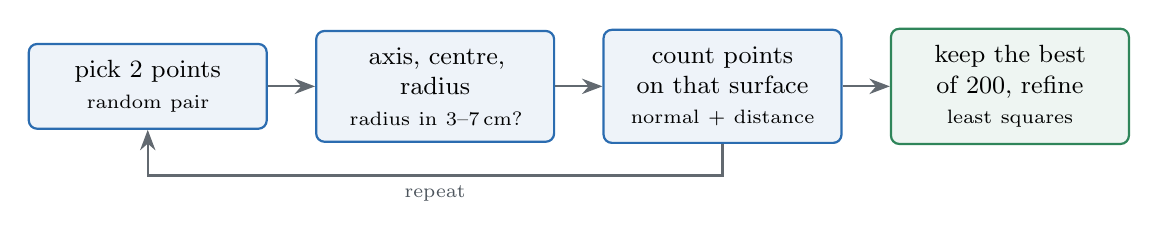
\begin{tikzpicture}[node distance=0.5cm and 0.6cm]
  \node[box=sky,text width=2.6cm] (a) {pick 2 points\\\scriptsize random pair};
  \node[box=sky,text width=2.6cm,right=of a] (b) {axis, centre,\\radius\\\scriptsize radius in 3--7\,cm?};
  \node[box=sky,text width=2.6cm,right=of b] (c) {count points\\on that surface\\\scriptsize normal + distance};
  \node[box=leaf,text width=2.6cm,right=of c] (d) {keep the best\\of 200, refine\\\scriptsize least squares};
  \draw[flow] (a) -- (b); \draw[flow] (b) -- (c); \draw[flow] (c) -- (d);
  \draw[flow] (c.south) -- ++(0,-0.4) -| node[lbl,pos=0.25,below]{repeat} (a.south);
\end{tikzpicture}
\end{center}

\textbf{End caps.} When a mug's flat base faces the camera squarely there is almost no wall to
see. If most normals agree, the points are flat, and the patch is \emph{round} with a mug-sized
radius, it is an \textbf{end cap} and the axis is its normal. ``Round'' matters: a flat strip
along a lying mug's side passed the first version of this test.

\noindent\begin{minipage}{\textwidth}
\centering
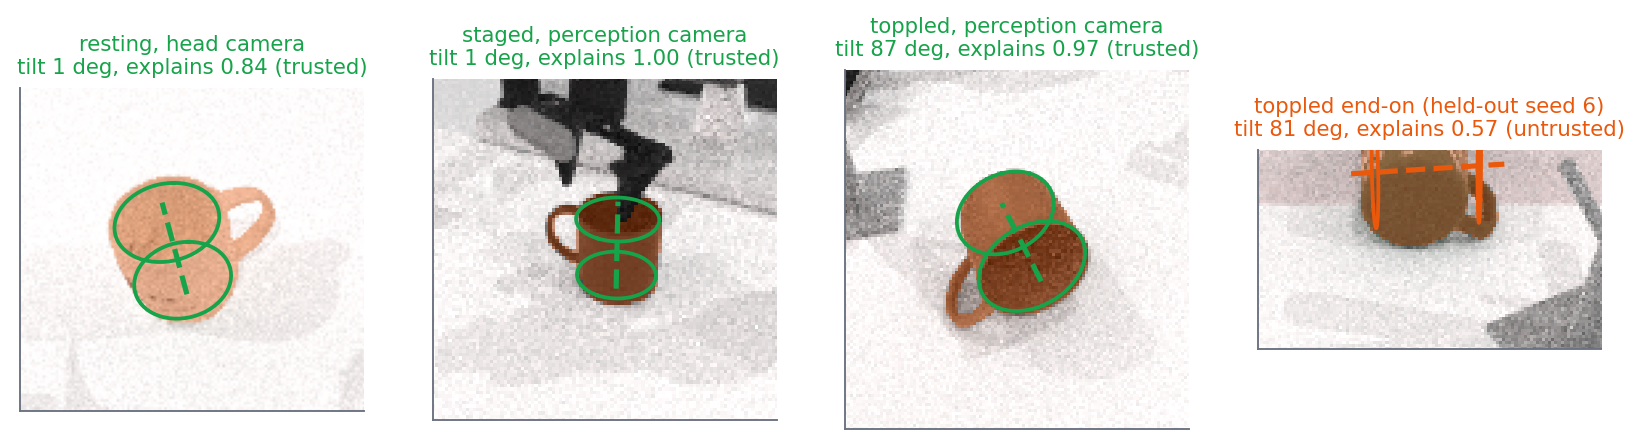
\includegraphics[width=\textwidth]{figures/fits_on_frames.png}\\[-2pt]
{\small Fitted cylinders drawn back onto real frames (orange = SAM 3 mask). Right: the held-out
end-on mug that fooled the old test. The fit reads it as lying down (81\textdegree), but it explains
only 57\% of its points, so it is not trusted (section~\ref{sec:trust}).}
\end{minipage}

% ================================================================ 6
\section{Removing the table, and a shadow}\label{sec:shadow}

Masks spill a little onto the table past the mug's edge. Points within 1\,cm of the table top
are dropped before fitting. This also fixed a detector mistake:

\begin{center}
\begin{minipage}{0.46\textwidth}
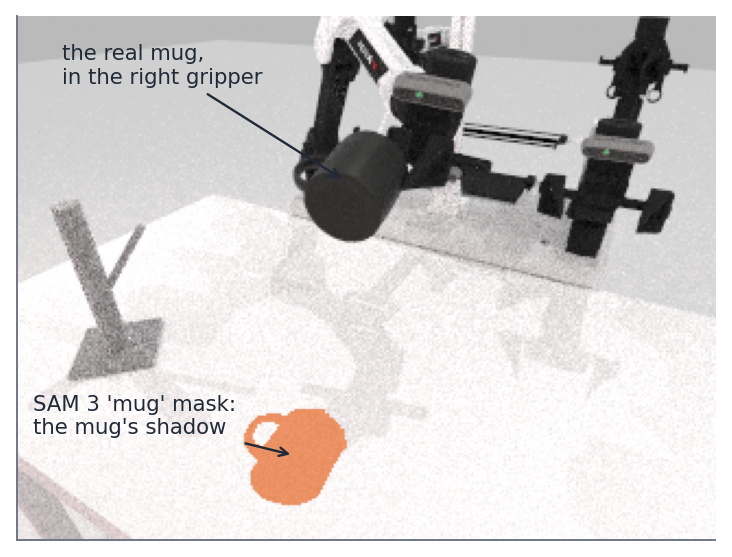
\includegraphics[width=\textwidth]{figures/shadow.png}
\end{minipage}\hfill
\begin{minipage}{0.5\textwidth}
Here SAM 3 labelled the mug's \textbf{shadow} as the mug, while the real mug was in the right
gripper. The shadow is flat and round, so it looked like an end cap standing upright.

Every shadow point lies on the table, so after the table points are removed nothing is left
to fit, and the pose is \emph{unknown}, which is the right answer.

\smallskip
\small The table height comes from the current frame's table mask, the same points the support
check already uses.
\end{minipage}
\end{center}

% ================================================================ 7
\section{Step 4: how much to trust a fit}\label{sec:trust}

A fit always returns \emph{some} cylinder. We need a number that says whether to believe it.
We use the share of the camera's mug points that the fitted cylinder \textbf{explains}: they lie
on its wall, or on a flat end inside its radius (the base, or the floor inside the cup).

\begin{center}
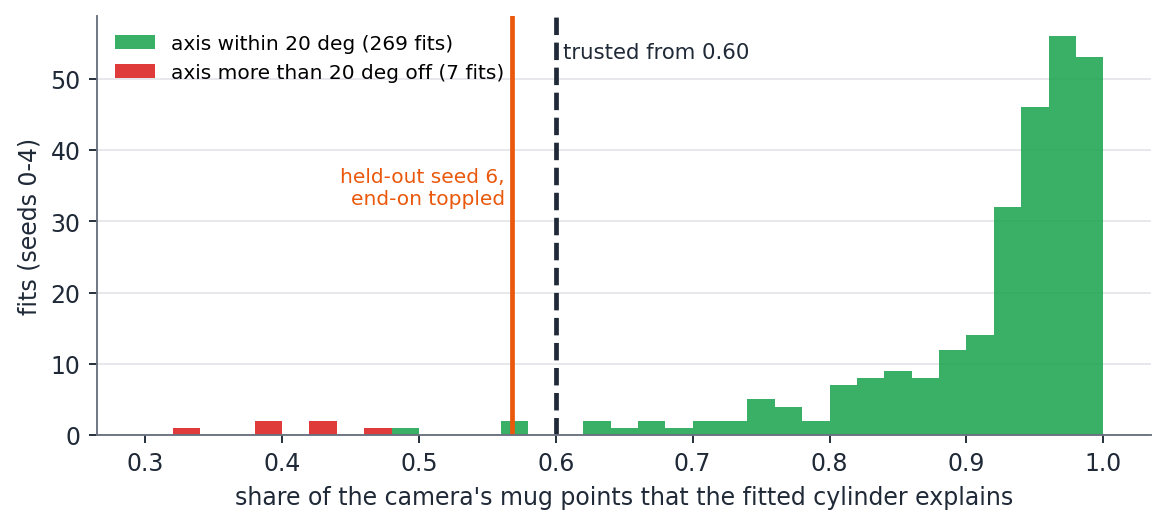
\includegraphics[width=0.92\textwidth]{figures/quality_gap.png}
\end{center}

On seeds 0--4 the wrong fits (red, all mugs half hidden by a gripper) explain 47\% of their
points or less. Almost all right fits explain far more. The floor of \textbf{0.60} sits in
that gap. This histogram uses every camera with a mug mask. In a real run the detector asks
only some cameras each phase; for those fits, every wrong fit was below 0.44 and every right
one above 0.70.

\subsection{Trusted and untrusted: an asymmetric rule}
The held-out end-on mug (orange line) was read correctly as lying down, but at 0.57 it fell
just below the floor and was thrown away, so the old test let it through.

Lowering the floor until it passed would be tuning on the test set. Instead we applied the
project's precision rule: \textbf{a reading that blocks an unsafe action needs less confidence
than one that allows it}.

\begin{center}
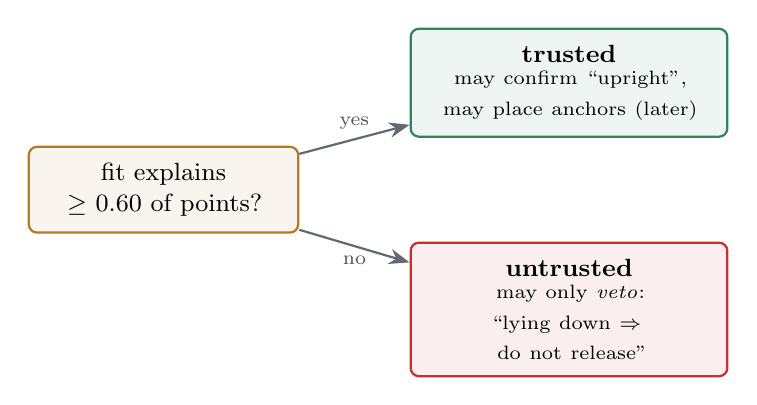
\begin{tikzpicture}[node distance=0.6cm and 1.0cm]
  \node[box=sun,text width=3cm] (fit) {fit explains\\$\ge$ 0.60 of points?};
  \node[box=leaf,text width=3.6cm,above right=0.1cm and 1.4cm of fit] (t) {\textbf{trusted}\\\scriptsize may confirm ``upright'',\\may place anchors (later)};
  \node[box=rose,text width=3.6cm,below right=0.1cm and 1.4cm of fit] (u) {\textbf{untrusted}\\\scriptsize may only \emph{veto}:\\``lying down $\Rightarrow$ do not release''};
  \draw[flow] (fit) -- node[lbl,above]{yes} (t);
  \draw[flow] (fit) -- node[lbl,below]{no} (u);
\end{tikzpicture}
\end{center}

A wrong veto costs a little recall: the supervisor waits. A wrong ``safe'' drops the mug.

\subsection{More than one camera}
Each camera is fitted on its own. Trusted fits must agree (axes within 15\textdegree, axis lines
within 3\,cm). If they disagree the pose is \emph{unknown} with reason \code{cameras_disagree};
we do not pick a favourite. The best-supported fit gives the pose.

% ================================================================ 8
\section{Placing the base}\label{sec:base}

\begin{center}
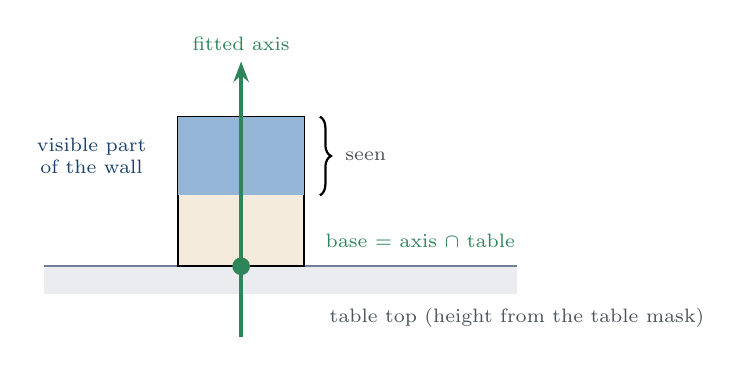
\begin{tikzpicture}[scale=1.0]
  \fill[stone!15] (-2.5,0) rectangle (3.5,-0.35);
  \draw[stone,thick] (-2.5,0) -- (3.5,0);
  \node[lbl,anchor=north west] at (1.0,-0.4) {table top (height from the table mask)};
  \draw[thick,fill=sun!15] (-0.8,0) rectangle (0.8,1.9);
  \fill[sky!50] (-0.8,0.9) rectangle (0.8,1.9);
  \node[lbl,text=sky!60!black] at (-1.9,1.4) {visible part\\of the wall};
  \draw[->,leaf,line width=1.4pt] (0,-0.9) -- (0,2.6) node[above,lbl,text=leaf]{fitted axis};
  \fill[leaf] (0,0) circle (3.2pt);
  \node[lbl,text=leaf,anchor=west] at (0.95,0.32) {base = axis $\cap$ table};
  \draw[decorate,decoration={brace,amplitude=4pt},thick] (1.0,1.9) -- (1.0,0.9);
  \node[lbl,anchor=west] at (1.2,1.4) {seen};
\end{tikzpicture}
\end{center}

If the axis is within 45\textdegree{} of vertical (the same cut-off the labels use for
``toppled'') and the lowest visible part comes within 3\,cm of the table, the mug stands on
the table. Its base centre is then where the axis meets the table top, \textbf{even though the
base itself is hidden}. That is what removed the 5.7\,cm height error.

Otherwise (lying down, or lifted) \code{base_known} is false and \code{position} is the middle
of the visible body. Which end of a lying mug is the base is step 6.

% ================================================================ 9
\section{Step 5: the release check uses the axis}

\begin{center}
\begin{tikzpicture}[node distance=0.45cm]
  \node[box=stone,text width=6.4cm] (s) {mug outline meets the local table?\\\scriptsize (unchanged)};
  \node[box=rose,text width=6.4cm,below=of s] (a) {\textbf{new:} any fitted axis tilted $>$45\textdegree?\\\scriptsize trusted or not $\to$ \code{False}, \code{mug_axis_tilted_not_upright}};
  \node[box=rose,text width=6.4cm,below=of a] (n) {visible surface faces up?\\\scriptsize median $|n_z| > 0.25 \to$ \code{False} (unchanged)};
  \node[box=sun,text width=6.4cm,below=of n] (u) {no surface test and no \emph{trusted} axis?\\\scriptsize $\to$ unknown};
  \node[box=leaf,text width=6.4cm,below=of u] (ok) {\code{True}: then the existing height and settle checks};
  \foreach \x/\y in {s/a,a/n,n/u,u/ok} \draw[flow] (\x) -- (\y);
\end{tikzpicture}
\end{center}

Either test can say ``not upright''. A trusted upright axis can also stand in for the surface
test when the mask was too small for it (the old ``sliver'' case).

% ================================================================ 10
\section{Results of steps 1--5}\label{sec:results15}

\begin{center}
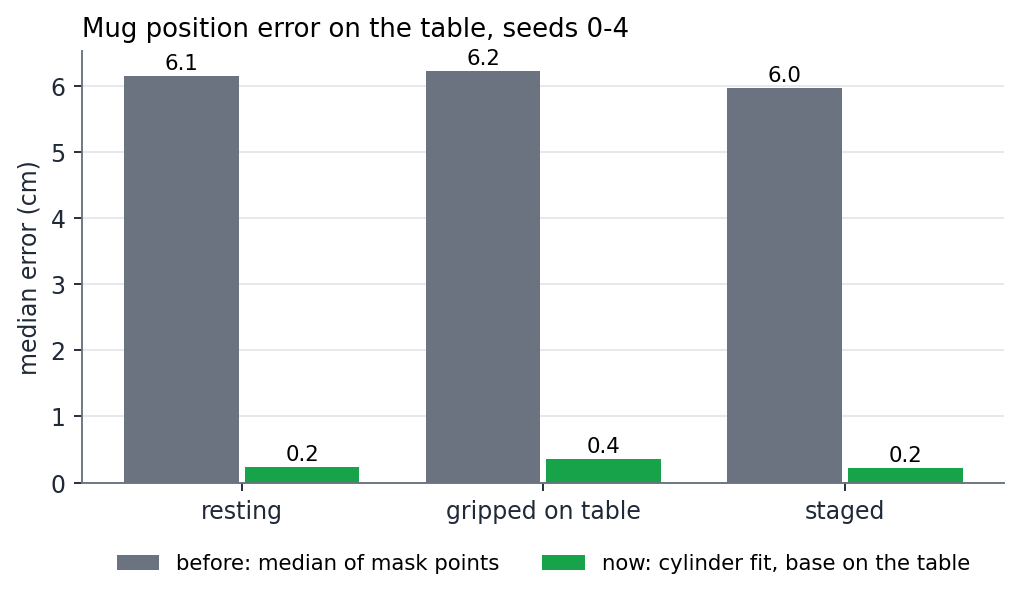
\includegraphics[width=0.8\textwidth]{figures/position_results.png}
\end{center}
\begin{center}
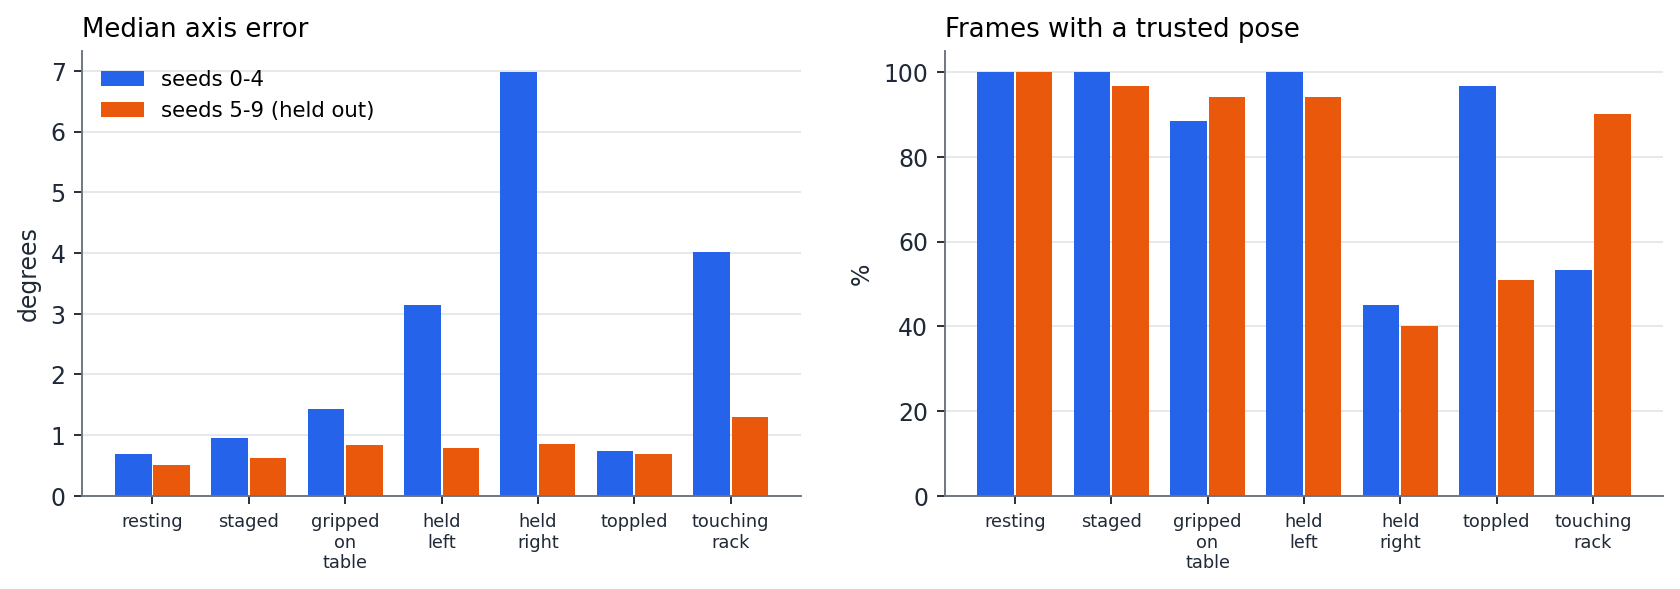
\includegraphics[width=\textwidth]{figures/axis_results.png}
\end{center}
\begin{center}
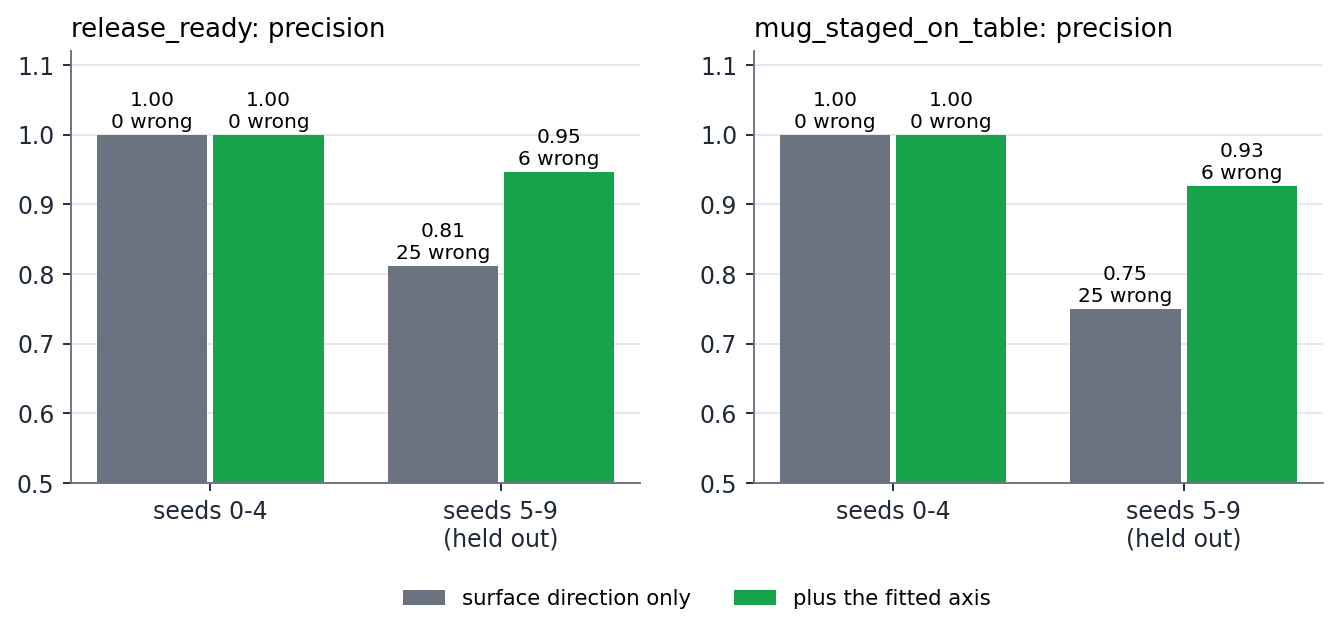
\includegraphics[width=0.9\textwidth]{figures/release_results.png}
\end{center}

\begin{center}
\small
\begin{tabularx}{\textwidth}{@{}Xrrrrr@{}}
\toprule
Run & Posed & Axis error & Base error & Up/toppled mix-ups & Confident wrong \\
\midrule
seeds 0--4, with perception camera & 159/216 & 1.1\textdegree & 2.6\,mm & 0 & 0 \\
seeds 0--4, without it & 98/216 & 1.5\textdegree & 2.5\,mm & 0 & 0 \\
seeds 5--9, with perception camera & 188/267 & 0.7\textdegree & 2.8\,mm & 0 & 0 \\
seeds 5--9, without it & 157/267 & 0.7\textdegree & 2.7\,mm & 0 & 0 \\
\bottomrule
\end{tabularx}
\end{center}

\begin{itemize}
  \item \textbf{No predicate lost anything}: every precision and recall on seeds 0--4 is identical
        to before.
  \item \textbf{Held-out ``safe to release'' false trues: 25 $\to$ 6}; precision 0.81 $\to$ 0.95.
  \item ``Posed'' counts trusted poses only. Most frames without one are mugs off the table or
        hidden by a gripper; the pose then says \emph{unknown} with a reason.
\end{itemize}

% ================================================================ 9b
\section{Step 6: which end is the base, which way is the handle}\label{sec:step6}

A mug standing on the table gets its base from the table (section~\ref{sec:base}). A mug lying
down, or held in the air, does not touch the table where we can use it. Without knowing
which end is the base, its axis could point either way, and a grasp or a re-stand would
turn it upside down.

\begin{center}
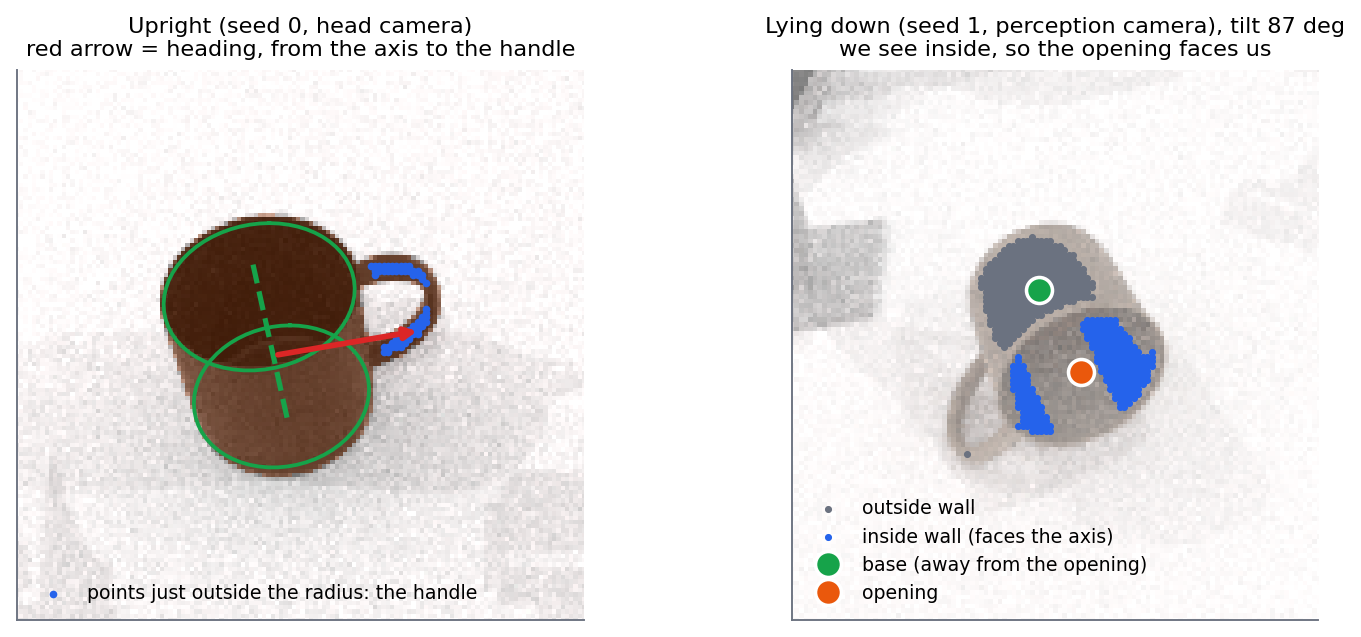
\includegraphics[width=\textwidth]{figures/handle_and_base.png}
\end{center}

\subsection{Two cues for the base end, which must agree}
\begin{center}
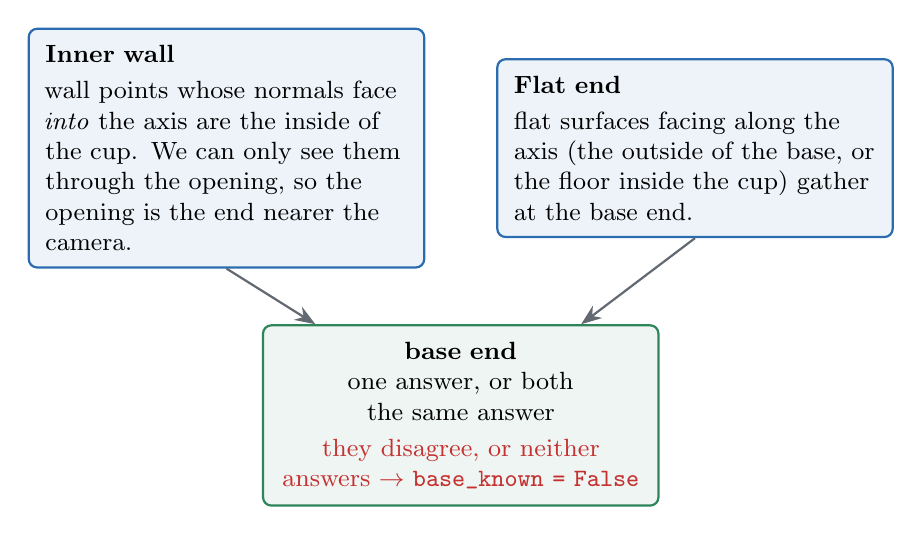
\begin{tikzpicture}[node distance=0.5cm and 0.9cm]
  \node[box=sky,text width=4.6cm,align=left] (inner) {\textbf{Inner wall}\\[2pt]\small wall points whose normals face
    \emph{into} the axis are the inside of the cup. We can only see them through the
    opening, so the opening is the end nearer the camera.};
  \node[box=sky,text width=4.6cm,align=left,right=of inner] (flat) {\textbf{Flat end}\\[2pt]\small flat surfaces facing
    along the axis (the outside of the base, or the floor inside the cup) gather at the base
    end.};
  \node[box=leaf,text width=4.6cm,below=0.9cm of $(inner.south)!0.5!(flat.south)$] (both) {\textbf{base end}\\\small one answer, or both the same answer\\[2pt]
    \textcolor{rose}{\small they disagree, or neither answers $\to$ \code{base_known = False}}};
  \draw[flow] (inner.south) -- (both);
  \draw[flow] (flat.south) -- (both);
\end{tikzpicture}
\end{center}
The inner-wall cue held in all 221 views on seeds 0--4 where at least a tenth of the wall faced
inwards. The flat-end cue alone failed on lying mugs, which is why there are two.

\subsection{Handle heading}
Handle points lie a little \emph{outside} the body: 0.8--3.5\,cm beyond the fitted radius,
within the body's height, all on one side. Their mean direction from the axis is the
\code{heading}. If they point in different directions (agreement below 0.8), no heading is given.
This test has a known weakness when the handle is hidden (section~\ref{sec:step8}).

\begin{center}
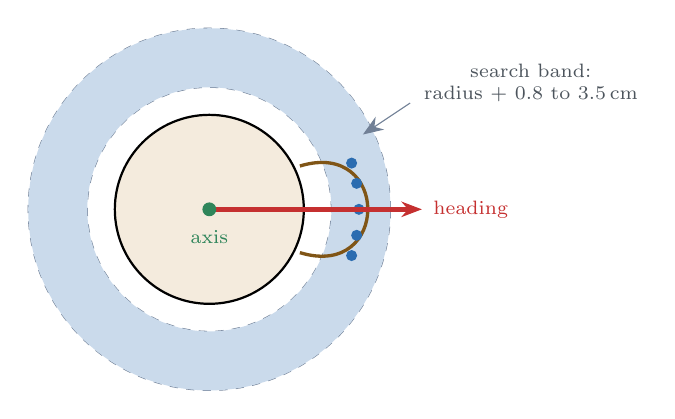
\begin{tikzpicture}[scale=1.0]
  \fill[sun!15] (0,0) circle (1.2);
  \draw[thick] (0,0) circle (1.2);
  \draw[dashed,stone] (0,0) circle (1.55);
  \draw[dashed,stone] (0,0) circle (2.3);
  \fill[sky!25,even odd rule] (0,0) circle (2.3) (0,0) circle (1.55);
  \draw[very thick,sun!70!black] (1.15,0.55) .. controls (2.3,0.9) and (2.3,-0.9) .. (1.15,-0.55);
  \foreach \a in {-18,-10,0,10,18} \fill[sky] (\a:1.9) circle (2pt);
  \draw[->,rose,line width=1.6pt] (0,0) -- (2.7,0) node[right,lbl,text=rose]{heading};
  \fill[leaf] (0,0) circle (2.5pt);
  \node[lbl,text=leaf] at (0,-0.35) {axis};
  \node[lbl,anchor=west] at (2.6,1.6) {search band:\\radius + 0.8 to 3.5\,cm};
  \draw[->,stone] (2.55,1.35) -- (1.95,0.95);
\end{tikzpicture}
\end{center}

\begin{center}
\small
\begin{tabularx}{\textwidth}{@{}Xrr@{}}
\toprule
 & Seeds 0--4 & Seeds 5--9 \\
\midrule
Lying mugs with a known base end & 25 of 28 & 28 of 28 \\
Base at the wrong end & 0 & 0 \\
Frames with a heading; median error (worst) & 66; 2.8\textdegree{} (11.9\textdegree) & 117; 2.8\textdegree{} (5.5\textdegree) \\
\bottomrule
\end{tabularx}
\end{center}

% ================================================================ 9c
\section{Step 7: the rack from depth}\label{sec:step7}

The rack is a vertical pole on a base plate with one slanted peg. That is two straight lines,
so the fit is two robust (RANSAC) line fits on the rack mask's points above the plate:

\begin{center}
\begin{tikzpicture}[node distance=0.5cm and 0.55cm]
  \node[box=grape,text width=2.4cm] (m) {rack mask\\\scriptsize points above\\the base plate};
  \node[box=sky,text width=2.4cm,right=of m] (p) {\textbf{pole line}\\\scriptsize within 15\textdegree{}\\of vertical};
  \node[box=sky,text width=2.4cm,right=of p] (g) {\textbf{peg line}\\\scriptsize points clear\\of the pole};
  \node[box=sun,text width=2.4cm,right=of g] (k) {key points\\\scriptsize foot, peg tip,\\peg seat};
  \node[box=leaf,text width=2.4cm,right=of k] (c) {\textbf{kept for the}\\\textbf{episode}\\\scriptsize once 2 views agree};
  \foreach \a/\b in {m/p,p/g,g/k,k/c} \draw[flow] (\a) -- (\b);
\end{tikzpicture}
\end{center}

\begin{center}
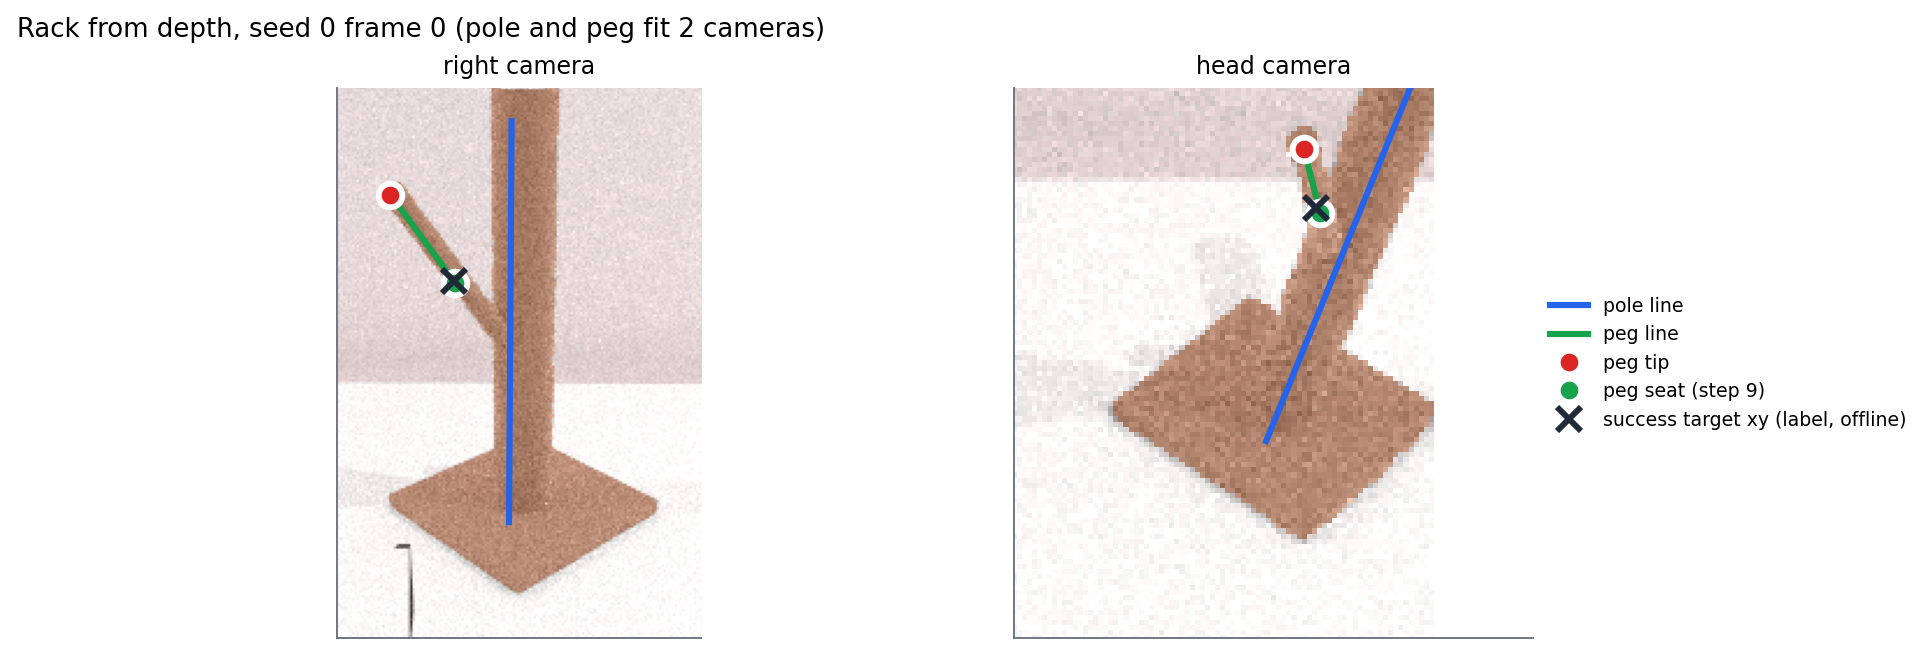
\includegraphics[width=\textwidth]{figures/rack_fit.png}
\end{center}

\begin{itemize}
  \item \textbf{Peg tip}: the far end of the peg line. Median error 2.9\,mm (seeds 0--4) and
        4.2\,mm (seeds 5--9), worst 1.4\,cm.
  \item \textbf{The rack does not move}, so its pose is fitted until it succeeds and then kept.
        After the review (section~\ref{sec:review}) it is kept only once \textbf{two views agree}
        on the peg tip within 2\,cm: two cameras in the same frame, or the same camera in two
        frames. One bad view (an arm across the peg, a stray mask) cannot fix a wrong hang
        target for the whole episode. It arrives at frame 0 or 16 in 9 of 10 episodes.
\end{itemize}

% ================================================================ 9d
\section{A second look: the code review}\label{sec:review}

Before wiring poses into the robot's targets, the branch was reviewed as a whole. What changed:

\begin{center}
\small
\begin{tabularx}{\textwidth}{@{}>{\raggedright\arraybackslash}p{4.2cm}X@{}}
\toprule
Finding & Change \\
\midrule
One rack fit decided the episode & two views must agree before the pose is kept \\
No table height, still a rack pose & no table, no rack pose: the plate's edge could pass for the peg \\
Key points could be edited & read-only, because one cached rack pose is shared by every later frame \\
Empty table mask crashed & guarded; the pose says \emph{unknown} \\
Normals computed on the whole image & only on the mask's bounding box: identical output on 320 real masks, 1.8$\times$ faster \\
\bottomrule
\end{tabularx}
\end{center}
Cost per frame after the review: about \textbf{32\,ms} for the mug pose; the rack fit, about
\textbf{164\,ms}, runs only until the rack pose is kept.

% ================================================================ 9e
\section{Step 9: aiming the arm with the poses}\label{sec:step9}

Steps 1--7 only \emph{describe} the scene. Step 9 lets the poses decide \emph{where the arm
goes}. Saved frames cannot show whether a different target makes a grasp or a hang succeed,
so this is behind a setting that is \textbf{off by default}. Pose estimation is judged by its
accuracy (section~\ref{sec:step8}); whether the new targets raise hanging success needs a live
comparison, which is follow-up work on the supervisor side. The rack results here were all
measured with the \code{explore_mug_rack} prompts, so that profile belongs with the setting:

\begin{cmd}
perception:\\
\ \ rgbd\_enabled: true\\
\ \ depth\_pose\_anchors: true \ \ \# needs -{}-perception-factory\\
\ \ rack\_prompt\_profile: explore\_mug\_rack
\end{cmd}

\subsection{What moves}
\begin{center}
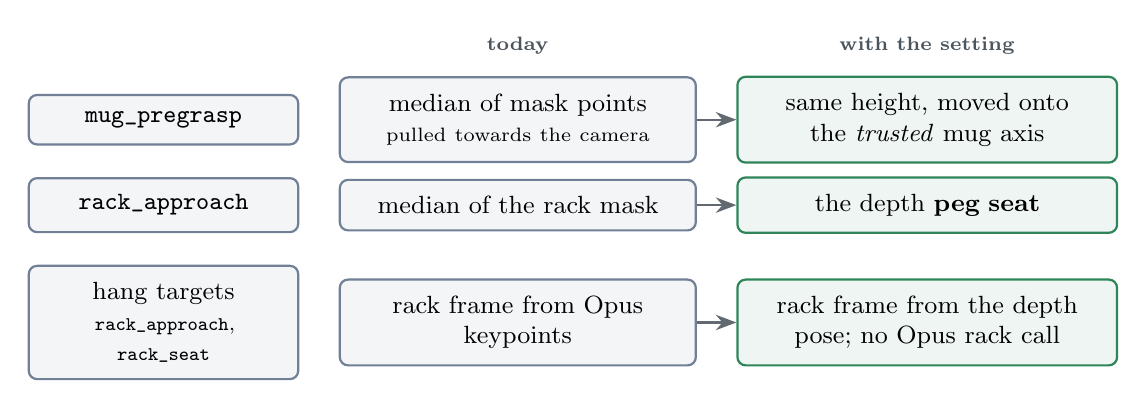
\begin{tikzpicture}[node distance=0.4cm and 0.5cm]
  \node[box=stone,text width=3.0cm] (t1) {\code{mug_pregrasp}};
  \node[box=stone,text width=4.1cm,right=of t1] (o1) {\small median of mask points\\\scriptsize pulled towards the camera};
  \node[box=leaf,text width=4.4cm,right=of o1] (n1) {\small same height, moved onto\\the \emph{trusted} mug axis};
  \node[box=stone,text width=3.0cm,below=of t1] (t2) {\code{rack_approach}};
  \node[box=stone,text width=4.1cm,right=of t2] (o2) {\small median of the rack mask};
  \node[box=leaf,text width=4.4cm,right=of o2] (n2) {\small the depth \textbf{peg seat}};
  \node[box=stone,text width=3.0cm,below=of t2] (t3) {hang targets\\\scriptsize \code{rack_approach}, \code{rack_seat}};
  \node[box=stone,text width=4.1cm,right=of t3] (o3) {\small rack frame from Opus\\keypoints};
  \node[box=leaf,text width=4.4cm,right=of o3] (n3) {\small rack frame from the depth\\pose; no Opus rack call};
  \node[lbl,above=0.15cm of o1] {\textbf{today}};
  \node[lbl,above=0.15cm of n1] {\textbf{with the setting}};
  \foreach \a/\b in {o1/n1,o2/n2,o3/n3} \draw[flow] (\a) -- (\b);
\end{tikzpicture}
\end{center}
Every new target \textbf{falls back} to today's target when its pose is missing (no trusted
mug pose, no confirmed rack pose). The mug-handle frame for the hang still comes from Opus.

\subsection{The peg seat: aim at what success is measured by}
RoboTwin counts a hang as done when the mug's handle is within 2\,cm (in xy) of the
\textbf{midpoint of the rack's base and the peg's end}, above a height floor, with the gripper
open. The peg \emph{tip} is the wrong place to aim: it is 2.4--3.5\,cm from that target. The
seat is the point \emph{on the peg} above the middle of the pole's foot and the peg tip.

\begin{center}
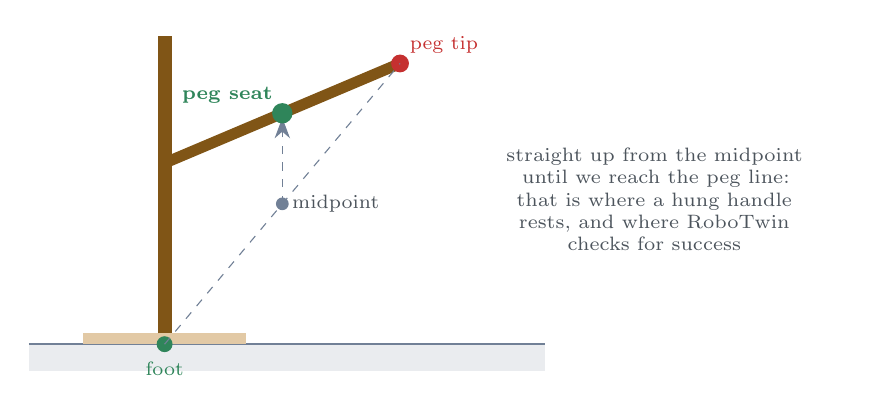
\begin{tikzpicture}[scale=1.15]
  \fill[stone!15] (-1.5,0) rectangle (4.2,-0.3);
  \draw[stone,thick] (-1.5,0) -- (4.2,0);
  \fill[sun!40] (-0.9,0) rectangle (0.9,0.12);
  \draw[line width=5pt,sun!70!black] (0,0.12) -- (0,3.4);
  \draw[line width=4pt,sun!70!black] (0,2.0) -- (2.6,3.1);
  \fill[leaf] (0,0) circle (2.5pt) node[below=3pt,lbl,text=leaf]{foot};
  \fill[rose] (2.6,3.1) circle (2.8pt) node[above right,lbl,text=rose]{peg tip};
  \draw[dashed,stone] (0,0) -- (2.6,3.1);
  \fill[stone] (1.3,1.55) circle (2pt) node[right,lbl]{midpoint};
  \draw[dashed,stone,->] (1.3,1.55) -- (1.3,2.5);
  \fill[leaf] (1.3,2.55) circle (3.2pt) node[above left,lbl,text=leaf]{\textbf{peg seat}};
  \node[lbl,anchor=west,text width=4.6cm] at (3.3,1.6) {straight up from the midpoint\\until we reach the peg line:\\that is where a hung handle\\rests, and where RoboTwin\\checks for success};
\end{tikzpicture}
\end{center}

\begin{center}
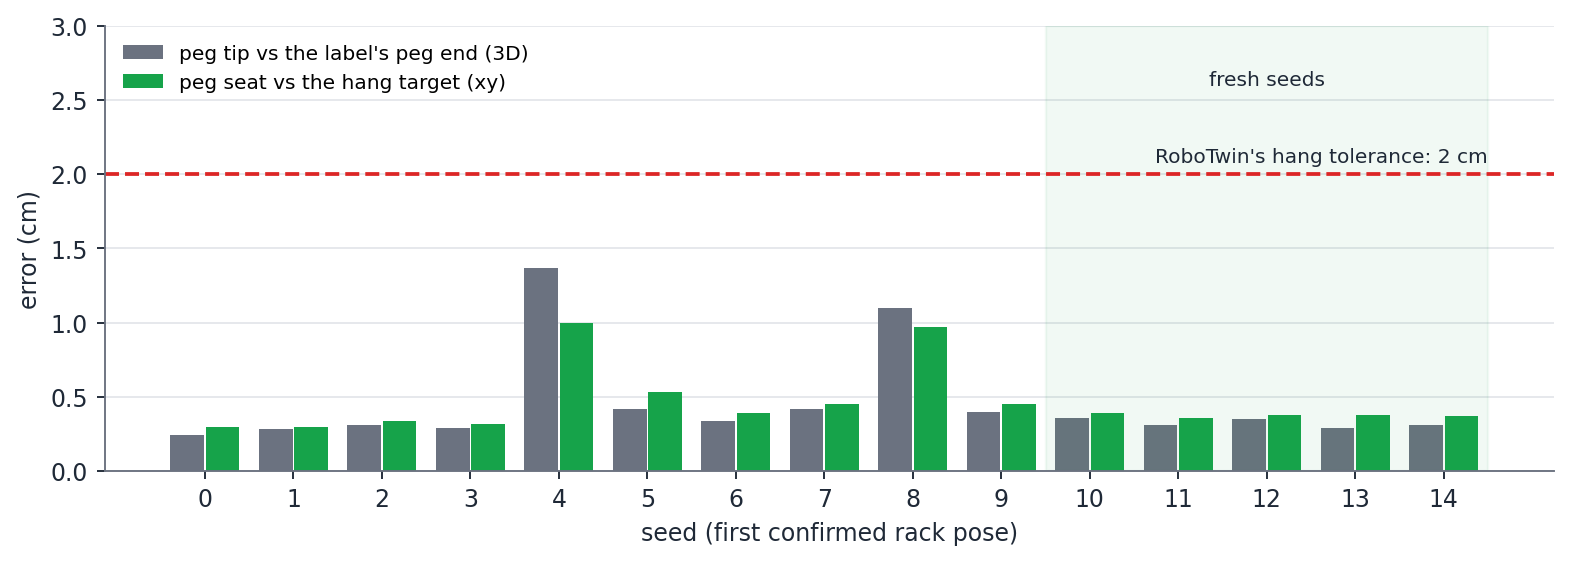
\includegraphics[width=\textwidth]{figures/seat_results.png}
\end{center}

\subsection{The rack frame for the hang}
The hang code already turns two frames (rack peg, mug handle) into gripper targets. The depth
rack frame copies the Opus keypoint frame's convention exactly, so that code did not change:
origin at the seat, $+x$ along the peg to its tip, $+y$ up the pole.

\begin{careful}
\textbf{Why the handle frame stays with Opus.} The depth handle point (the median of the handle's
visible points) is 1.7--2.1\,cm from the label's handle point, and a hang must land within
2\,cm. It is tracked in the evaluator (\code{handle_point_error_m}) for later work, not used.
\end{careful}

\begin{changeit}
\begin{itemize}[leftmargin=*]
  \item \code{object_pose.py}: \code{_peg_seat}, the \code{peg_seat} key point.
  \item \code{grounding.py}: \code{bind_pose_approach_anchor}; \code{episode_rack_pose}.
  \item \code{hang_targets.py}: \code{rack_frame_from_pose}, \code{DepthRackFrame}.
  \item \code{pose_grounding.py}: \code{frame_from_axes}, shared with the Opus keypoint path.
  \item \code{preparation.py}, \code{runtime/settings.py}, \code{runtime/assembly.py}, \code{run_skills.py}: the setting.
\end{itemize}
\end{changeit}

% ================================================================ 8
\section{Step 8: a clean test on fresh seeds}\label{sec:step8}

Seeds 0--4 were used for tuning and seed 6 was inspected while designing the trust rule, so
neither can say whether the method holds up. Seeds 10--14 were captured after the code was
frozen at commit \code{4257459}, and scored once. \textbf{Nothing was changed after seeing them.}

\begin{center}
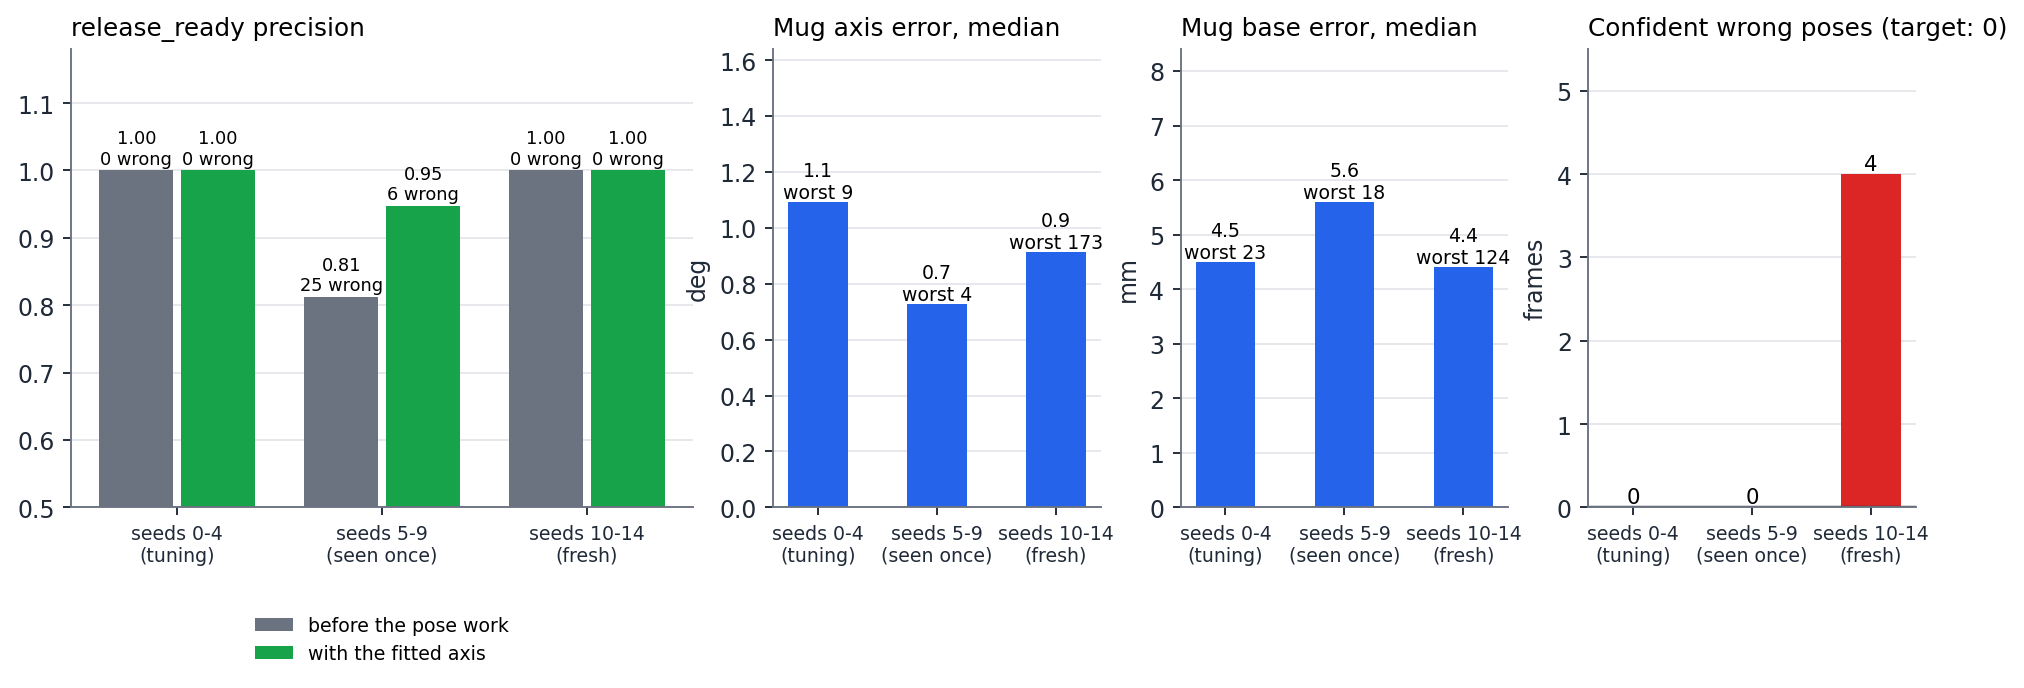
\includegraphics[width=\textwidth]{figures/fresh_results.png}
\end{center}

\subsection{Against the targets set in the plan}
\begin{center}
\small
\begin{tabularx}{\textwidth}{@{}Xrrc@{}}
\toprule
Measure (seeds 10--14, 290 frames) & Target & Result & \\
\midrule
Mug base error, median / 90th percentile & 1.5 / 3\,cm & 0.44 / 1.66\,cm & \textcolor{leaf}{\faCheck} \\
Mug axis error, median & 10\textdegree & 0.9\textdegree & \textcolor{leaf}{\faCheck} \\
Upright/toppled mix-ups & 0 & 0 & \textcolor{leaf}{\faCheck} \\
Handle heading error, median & 20\textdegree & 2.9\textdegree & \textcolor{leaf}{\faCheck} \\
Rack peg tip error, median (worst) & 1\,cm & 3.1\,mm (3.6\,mm) & \textcolor{leaf}{\faCheck} \\
\textbf{Confident wrong poses} & \textbf{0} & \textbf{4} & \textcolor{rose}{\faTimes} \\
\bottomrule
\end{tabularx}
\end{center}

The plan said the confirmation must state how much toppled evidence it holds: \textbf{71 toppled
frames} (seed 10: 19, seed 13: 29, seed 14: 23), with the base end known in 48 of them. The median
base error on those is 1.6\,cm, larger than the 4--6\,mm over all poses, because a lying mug's base
is placed where its visible points end.

\subsection{The four failures}
\begin{center}
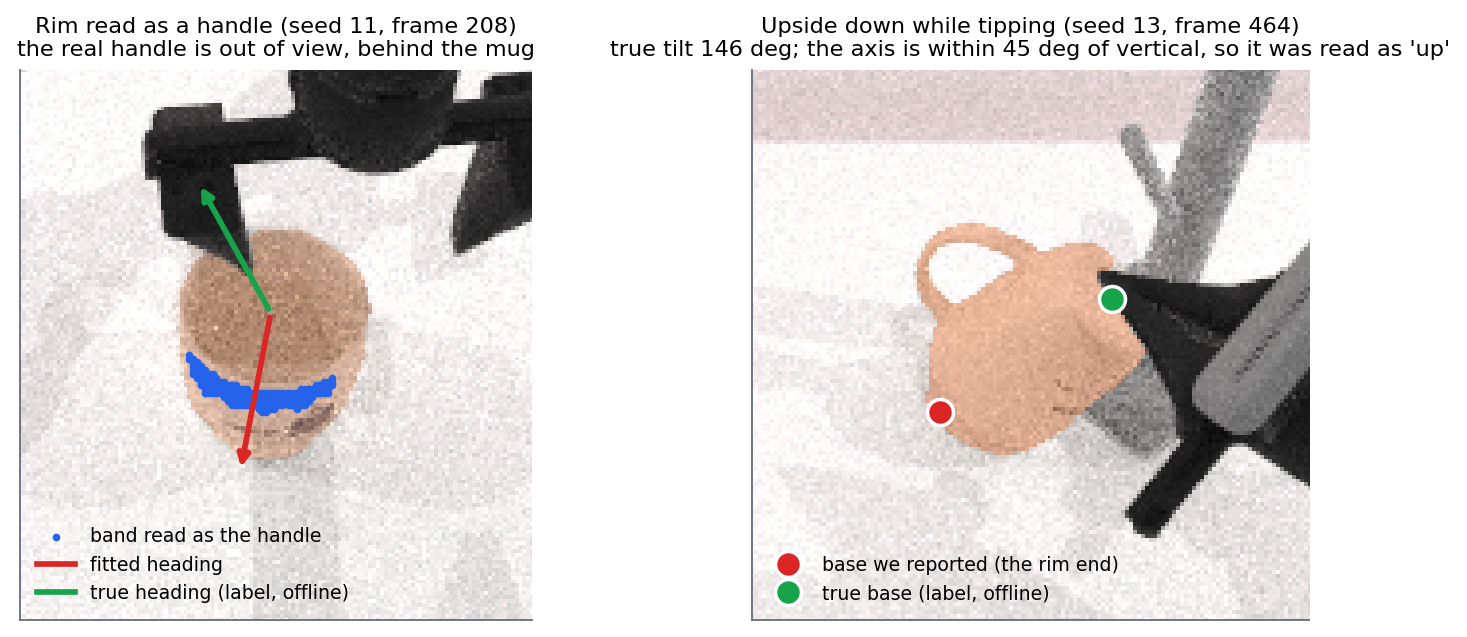
\includegraphics[width=\textwidth]{figures/fresh_failures.png}
\end{center}

\begin{center}
\small
\begin{tabularx}{\textwidth}{@{}>{\raggedright\arraybackslash}p{3.1cm}>{\raggedright\arraybackslash}X>{\raggedright\arraybackslash}X@{}}
\toprule
Frames & What happened & Effect today \\
\midrule
3 frames: seeds 11 and 13, mug model 4 & With the handle out of view, a band of points near the
rim sits just outside the fitted radius, on the camera side. It reads as a handle pointing at the
camera: 145--168\textdegree{} off. Axis and base are correct (3\,mm). & None: no decision reads the
heading yet. A recovery skill choosing a grip side from it would be misled. \\
1 frame: seed 13, frame 464 & The mug was upside down while tipping (146\textdegree). Its axis was
within 45\textdegree{} of vertical, and the code assumes such a mug has its base at the bottom. The
base landed on the rim end, 12\,cm off. & None: the frame was not called safe to release, and the
mug approach uses the axis \emph{line}, which is unaffected by the flip. \\
\bottomrule
\end{tabularx}
\end{center}

\begin{careful}
\textbf{These are not patched.} A fix made after looking at fresh seeds would spoil them as a test,
which is what happened to seed 6. The proposed fixes are below (section~\ref{sec:open}); they
should be tuned on seeds 0--4 and confirmed on a new set of seeds.
\end{careful}

\subsection{The release check on fresh seeds}
\begin{center}
\small
\begin{tabularx}{\textwidth}{@{}Xrrrr@{}}
\toprule
Seeds 10--14 & \multicolumn{2}{c}{With perception camera} & \multicolumn{2}{c}{Head and wrists only} \\
 & before & after & before & after \\
\midrule
\code{release_ready} precision & 1.00 & 1.00 & 1.00 & 1.00 \\
\code{release_ready} recall & 0.61 & 0.62 & 0.52 & 0.52 \\
\code{mug_staged_on_table} recall & 0.53 & 0.54 & 0.47 & 0.47 \\
\code{mug_lifted} recall & 0.86 & 0.86 & 0.74 & 0.74 \\
\code{right_mug_lifted} recall & 0.95 & 0.95 & 0.53 & 0.53 \\
False ``true'', any predicate & 0 & 0 & 0 & 0 \\
\bottomrule
\end{tabularx}
\end{center}

The pose work did no harm, but this test \textbf{neither confirms nor refutes} the earlier gain
(25 $\to$ 6 wrong on seeds 5--9): none of the fresh seeds produced the end-on mug that fools the old
surface test, so there was nothing for the veto to catch. That gain still rests on seeds we looked at.

\subsection{Which cameras a live run actually has}
The ``with perception camera'' numbers need a caveat. The fixed perception camera exists only
in the capture tools; \code{run_skills.py} does not add it. Each observation, SAM 3 looks at the
\textbf{head camera}, and tries another camera only if the head finds no confident mug
(the wrist for the phase) or, with the \code{explore_mug_rack} profile, no clear rack (the right wrist).
\textbf{Today's live runs match the blue bars.}

\begin{center}
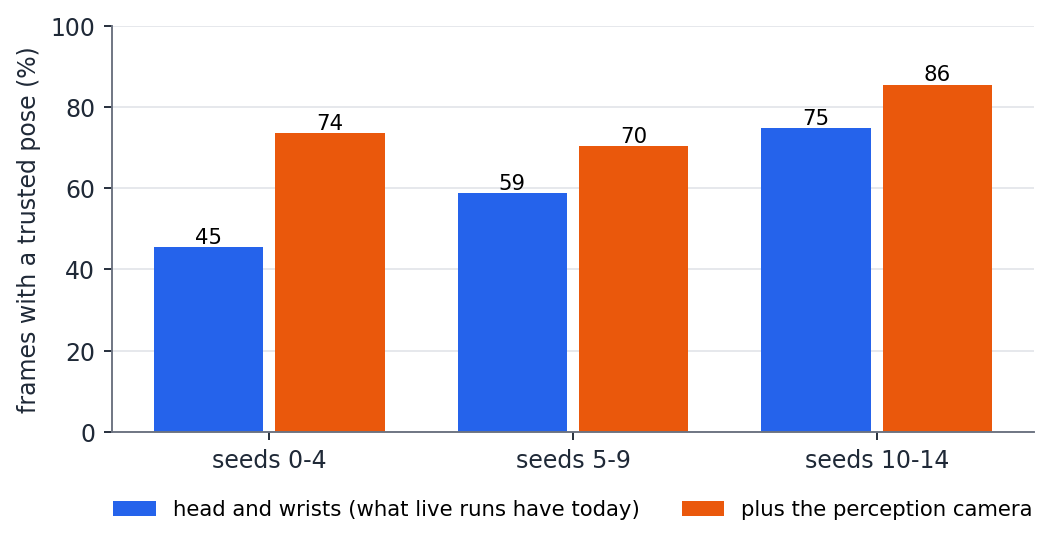
\includegraphics[width=0.74\textwidth]{figures/camera_coverage.png}
\end{center}

Adding the camera mainly buys coverage. Replaying each order on the cached answers (483 frames,
seeds 0--9, mug detections only) shows it hardly changes the number of SAM 3 calls:

\begin{center}
\small
\begin{tabularx}{\textwidth}{@{}Xrr@{}}
\toprule
Camera order & Calls per frame & Mug found \\
\midrule
Head, then wrist (today) & 1.69 & 61\% \\
Head, then perception, then wrist & 1.75 & 82\% \\
Perception, then head, then wrist & 1.62 & 82\% \\
Perception, then wrist & 1.51 & 74\% \\
\bottomrule
\end{tabularx}
\end{center}

% ================================================================ S
\section{What this means for supervising the task}\label{sec:supervision}

The supervisor does not move the robot itself. It watches, decides and checks: the planner
picks the next skill (move to an anchor, grasp, release), the frozen policy runs it, and
predicates read the cameras to say whether a phase is done or whether it is safe to go on.
Supervision is only as good as what it can \emph{see}. Before this work it saw ``a mug-coloured
blob, roughly here''. Now it sees an object with a base, an axis, a handle and a rack peg,
and it knows when it does not know.

\begin{center}
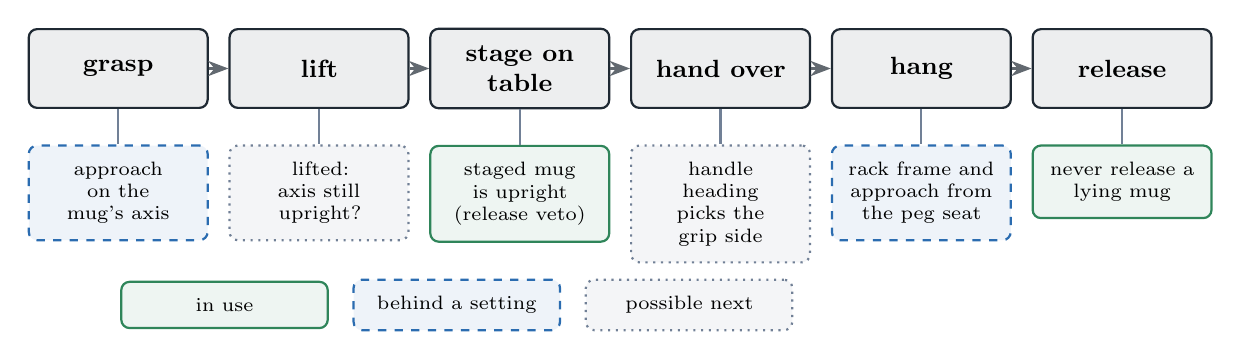
\begin{tikzpicture}[node distance=0.25cm]
  \tikzset{phase/.style={box=ink,text width=1.85cm,minimum height=1.0cm,font=\small\bfseries}}
  \node[phase] (p1) {grasp};
  \node[phase,right=of p1] (p2) {lift};
  \node[phase,right=of p2] (p3) {stage on\\table};
  \node[phase,right=of p3] (p4) {hand over};
  \node[phase,right=of p4] (p5) {hang};
  \node[phase,right=of p5] (p6) {release};
  \foreach \a/\b in {p1/p2,p2/p3,p3/p4,p4/p5,p5/p6} \draw[flow] (\a) -- (\b);

  \tikzset{now/.style={box=leaf,text width=1.85cm,font=\scriptsize,align=center},
           opt/.style={box=sky,text width=1.85cm,font=\scriptsize,align=center,dashed},
           later/.style={box=stone,text width=1.85cm,font=\scriptsize,align=center,dotted}}
  \node[opt,below=0.45cm of p1] (a1) {approach on the\\mug's axis};
  \node[later,below=0.45cm of p2] (a2) {lifted: axis still\\upright?};
  \node[now,below=0.45cm of p3] (a3) {staged mug\\is upright\\(release veto)};
  \node[later,below=0.45cm of p4] (a4) {handle heading\\picks the grip side};
  \node[opt,below=0.45cm of p5] (a5) {rack frame and\\approach from\\the peg seat};
  \node[now,below=0.45cm of p6] (a6) {never release a\\lying mug};
  \foreach \p/\a in {p1/a1,p2/a2,p3/a3,p4/a4,p5/a5,p6/a6} \draw[thick,stone] (\p) -- (\a);

  \node[now,text width=2.2cm,below=0.5cm of a2,xshift=-1.2cm] (k1) {in use};
  \node[opt,text width=2.2cm,right=0.3cm of k1] (k2) {behind a setting};
  \node[later,text width=2.2cm,right=0.3cm of k2] (k3) {possible next};
\end{tikzpicture}
\end{center}

\subsection{Five things the supervisor gains}
\begin{enumerate}
  \item \textbf{A release gate that is harder to fool} \textcolor{leaf}{(measured)}. A wrong
        ``safe to release'' is the worst predicate mistake: the mug drops or tips, and the task
        usually cannot recover. The fitted axis vetoes it even when the fit is only partly
        trusted (section~\ref{sec:trust}). Wrong answers fell from 25 to 6 on seeds 5--9; on the
        fresh seeds there were none before or after (section~\ref{sec:step8}).
  \item \textbf{Failure states it can recognise} \textcolor{leaf}{(measured)}. ``The mug has
        toppled'' is now read from the axis: no upright/toppled mix-ups on any of the 15 seeds,
        and on the fresh seeds the base end is known in 48 of 71 toppled frames. A recovery skill
        could use this, but none does yet, and a lying mug's handle is rarely seen.
  \item \textbf{Targets that match what is checked} \textcolor{sun}{(accuracy measured, benefit
        expected)}. RoboTwin judges the hang at the peg seat, not the peg tip. The seat is
        3--5\,mm from the success target, where the tip is 2.4--3.5\,cm from it. The mug
        approach no longer aims at a point pulled 2\,cm towards the camera. Whether this
        raises hanging success has not been run.
  \item \textbf{One model call fewer} \textcolor{sun}{(behind the setting)}. The rack frame for the hang came from Opus keypoints:
        a network call to a large model, with its latency and cost. With the
        setting on, it comes from depth, about 0.16\,s per try until two views agree, and is
        then kept for the episode.
  \item \textbf{\emph{Unknown} with a reason.} Every pose carries \code{trusted} and a
        \code{reason} (\code{cameras_disagree}, \code{cylinder_fit_inliers_low},
        \code{rack_fit_awaiting_confirmation}, \dots). The supervisor can respond to the reason:
        look again from another camera, wait for the arm to clear the view, or fall back to
        the old target, instead of acting on a guess.
\end{enumerate}

\subsection{How the supervisor should read a pose}
\begin{center}
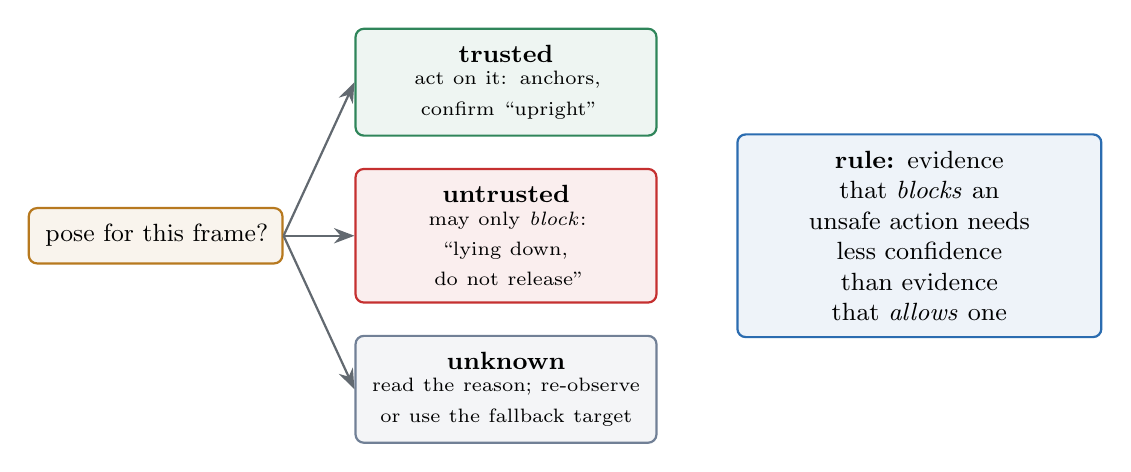
\begin{tikzpicture}[node distance=0.55cm and 0.9cm]
  \node[box=sun,text width=2.8cm] (q) {pose for this frame?};
  \node[box=leaf,text width=3.4cm,right=of q,yshift=1.95cm] (t) {\textbf{trusted}\\\scriptsize act on it: anchors,\\confirm ``upright''};
  \node[box=rose,text width=3.4cm,right=of q] (u) {\textbf{untrusted}\\\scriptsize may only \emph{block}:\\``lying down, do not release''};
  \node[box=stone,text width=3.4cm,right=of q,yshift=-1.95cm] (n) {\textbf{unknown}\\\scriptsize read the reason; re-observe\\or use the fallback target};
  \draw[flow] (q.east) -- (t.west);
  \draw[flow] (q.east) -- (u.west);
  \draw[flow] (q.east) -- (n.west);
  \node[box=sky,text width=4.2cm,right=1.0cm of u] (r) {\small \textbf{rule:} evidence that \emph{blocks} an\\
    unsafe action needs less confidence\\than evidence that \emph{allows} one};
\end{tikzpicture}
\end{center}

\subsection{What the planner can and cannot infer}
\begin{center}
\small
\begin{tabularx}{\textwidth}{@{}>{\raggedright\arraybackslash}X>{\raggedright\arraybackslash}X@{}}
\toprule
\textcolor{leaf}{\faCheck}\ \textbf{Can} & \textcolor{rose}{\faTimes}\ \textbf{Cannot (yet)} \\
\midrule
whether the mug stands or lies, and where its base is (mm) &
the mug's pose while a gripper hides most of it: only 40--60\% of right-hand-held frames get a trusted pose \\
which end of a lying mug is the base & the handle's exact position: about 2\,cm off, too coarse to hang by \\
the handle direction of a standing mug when the handle is in view (about 3\textdegree) & whether the handle is \emph{on} the peg: the hang itself is still checked by RoboTwin; nor a hidden handle's direction, which can be misread \\
where the hung handle must end up on the rack (3--5\,mm) & which end is the base of an upside-down mug near vertical; anything about objects with no spec \\
\bottomrule
\end{tabularx}
\end{center}

% ================================================================ 11
\section{What is still open}\label{sec:open}

\begin{careful}
\begin{itemize}[leftmargin=*]
  \item \textbf{The ``no confident wrong poses'' target failed on fresh seeds} (4 of 290 frames).
        Neither cause affects a decision today. Both need fixing before anything relies on them:
        \begin{itemize}[leftmargin=*]
          \item \emph{Rim read as a handle:} require the handle points to span part of the mug's height, which a thin rim band does not.
          \item \emph{Upside-down near vertical:} use the base-end cues on tilted mugs too, and report \emph{base unknown} when they disagree with ``up''.
        \end{itemize}
  \item \textbf{The release gain is unconfirmed.} The 25 $\to$ 6 result is from seeds 5--9, and the
        fresh seeds held no case that tests it. Its 6 remaining wrong answers are all seed 6's
        end-on mug.
  \item \textbf{Held mugs are often unknown.} Gripper points are not removed, because the
        measured hand pose sits about 0.2\,m behind the fingers and a box around it would delete
        the mug. On the fresh seeds, 59\% of right-hand-held frames get a trusted pose.
  \item \textbf{The depth handle point is too coarse to hang by}: 2.9\,cm median on the fresh seeds.
        The handle frame stays with Opus.
  \item \textbf{Live results do not exist.} \code{depth_pose_anchors} has never run in a live
        episode. The rack may also be confirmed late (seed 10: frame 112), and targets
        fall back until then.
\end{itemize}
\end{careful}

\begin{center}
\begin{tikzpicture}[node distance=0.35cm]
  \node[box=leaf,text width=2.3cm] (s5) {\faCheck\ steps 1--5\\\scriptsize mug pose and\\release veto};
  \node[box=leaf,text width=2.3cm,right=of s5] (s6) {\faCheck\ steps 6--7\\\scriptsize base end, handle,\\rack peg};
  \node[box=leaf,text width=2.3cm,right=of s6] (s9) {\faCheck\ step 9\\\scriptsize targets, behind\\a setting};
  \node[box=sun,text width=2.3cm,right=of s9] (s8) {step 8\\\scriptsize fresh seeds: 5 of\\6 targets met};
  \node[box=stone,text width=2.3cm,right=of s8,dashed] (n) {follow-up\\\scriptsize fix the 2 causes;\\live comparison};
  \foreach \x/\y in {s5/s6,s6/s9,s9/s8,s8/n} \draw[flow] (\x) -- (\y);
\end{tikzpicture}
\end{center}

% ================================================================ 12
\section{Commands}

Run from the repository root. Scoring needs no GPU once the SAM 3 answers are cached.

\textbf{Tests} (CPU, seconds):
\begin{cmd}
conda run -n robotwin python -m pytest -q tests/test\_object\_pose.py \textbackslash\\
\ \ tests/test\_perception\_grounding.py tests/test\_perception\_scoring.py
\end{cmd}

\textbf{Score poses and predicates} (under a minute per five seeds):
\begin{cmd}
conda run -n robotwin python -m development.replays.perception\_evaluation \textbackslash\\
\ \ -{}-frames data/perception/frames\_cam/seed\_0 \textbackslash\\
\ \ ... (one -{}-frames per seed, up to seed\_4) \textbackslash\\
\ \ -{}-output data/perception/reports/pose\_dev\_with\_camera
\end{cmd}
Add \texttt{-{}-ignore-camera perception\_camera} to score without the new camera. The report's
\texttt{summary.md} has a ``Mug pose by state'' table; \texttt{frames.jsonl} has the per-frame
pose errors and reasons.

\needspace{10\baselineskip}
\textbf{Repeat the fresh-seed test.} Cache each capture once (it resumes if interrupted), then
score from a checkout of the frozen commit \code{4257459}:
\begin{cmd}
python -m development.replays.sam3\_cache -{}-frames data/perception/frames\_fresh/seed\_10\\
python -m development.replays.perception\_evaluation \textbackslash\\
\ \ -{}-frames data/perception/frames\_fresh/seed\_10 ... (up to seed\_14) \textbackslash\\
\ \ -{}-output data/perception/reports/fresh\_with\_camera
\end{cmd}

\needspace{8\baselineskip}
\textbf{Rebuild this guide}:
\begin{cmd}
conda run -n robotwin env PYTHONPATH=\$PWD python \textbackslash\\
\ \ docs/Collaboration/Olusola/guides/pose\_estimation/make\_figures.py\\
cd docs/Collaboration/Olusola/guides/pose\_estimation \&\& \textbackslash\\
\ \ conda run -n texbuild tectonic -X compile pose\_estimation\_guide.tex
\end{cmd}

\begin{changeit}
Read next: \code{plans/pose_estimation_plan.md} (the full plan and its progress notes) and
\code{guides/perception/perception_guide.pdf} (how predicates and the provider work).
\end{changeit}

\end{document}
